%!TEX root = 0.tex

\documentclass[a4paper,11pt]{article}

\usepackage{color}
%\usepackage{graphics}

\usepackage{pstricks,pst-node,pst-tree}


%\usepackage{times}
%\usepackage{mathptmx}



\usepackage{amsmath,amsthm,amssymb,amscd,amsfonts}
\usepackage{mychicago,url,umlaut,latexsym}
\usepackage{graphicx}


%\usepackage{picin/picins}



%% \usepackage{pst-tree,pst-node}
%% \usepackage{amsmath,amsthm,amssymb,amscd,amsfonts}
%% \usepackage{mychicago,covington,url,umlaut,latexsym}
%\usepackage{graphicx} %[dvips]
%% %\usepackage{epsfig}
%% %\usepackage{german}

%\usepackage{covington}
\makeatletter
\newcounter{@@equationsave}
\newenvironment{examples}{%
  \begin{list}{(\theequation)}{%
      \setcounter{@@equationsave}{\arabic{equation}}%
      \usecounter{equation}%
      \setcounter{equation}{\arabic{@@equationsave}}% 
      \def\makelabel##1{##1\hfil}}}{
  \end{list}}
%\newenvironment{example}{\begin{examples}\item}{\end{examples}}
\makeatother








\input local-macros
\usepackage{tree-macros}




\newcommand\ie{\textit{i.e.}\xspace}
\newcommand\eg{\textit{e.g.}\xspace}

\theoremstyle{plain}
\newtheorem{theorem}{Theorem}
\newtheorem{prop}[theorem]{Proposition}
\newtheorem{kor}[theorem]{Corollary}
\newtheorem{lemma}[theorem]{Lemma}
\newtheorem{verm}{Conjecture}

\theoremstyle{definition}
\newtheorem{definition}[theorem]{Definition}
\newtheorem{bem}{Remark}


\sloppy 
\pagestyle{headings}

% Laengen aus Joachims Dissertation
\setlength{\evensidemargin}{.75cm}      % linker und rechter Rand
\setlength{\oddsidemargin}{.75cm}               
\setlength{\marginparwidth}{1.5cm}
\setlength{\marginparsep}{0.8cm}

\setlength{\topmargin}{0cm}             % oberer Rand
\setlength{\textwidth}{14.8cm}
\setlength{\textheight}{21cm}

\setlength{\parindent}{0pt}
\setlength{\parskip}{1.5ex}

\setcounter{tocdepth}{1}             % hoechstens Sections im TOC

\hyphenation{Fach-be-reich}

\title{Utool: The Swiss Army Knife of Underspecification \\ Version 3.1}
\author{Alexander Koller\thanks{Currently at Columbia University.} \ and Stefan Thater \\
SFB 378, Project CHORUS \\
Saarland University, Saarbr\"ucken, Germany \\
\url{{koller|stth}@coli.uni-sb.de}}
\date{\today}


\newcommand{\utool}{utool}


%%%%%%%%%%% HEVEA support %%%%%%%%%%%%%%%%%%%

%HEVEA \newstyle{PRE}{text-align:left;align:center;margin-top:5ex;margin-bottom:5ex;margin-left:auto;margin-right:auto;padding-top:2ex;padding-left:2em;padding-bottom:2ex;width:60em;background-color:\#DDDDDD}

%HEVEA \newcommand{\citeauthoryear}[1]{\cite{#1}}
%HEVEA \newcommand{\todo}[1]{\textbf{#1}}
%HEVEA \newcommand{\strut}{}
%HEVEA \newcommand{\citeN}[1]{\cite{#1}}




\begin{document}

\maketitle


\todo{
\begin{itemize}
\item begriffe, die besser erklaert gehoeren:
\begin{itemize}
\item solved form
\item utool vs.\ domgraph (bild malen?)
\end{itemize}
\item dinge, die noch keinen platz haben:
\begin{itemize}
\item redundanzeliminierung
\end{itemize}

\end{itemize}
}


\section{Introduction}  \label{sec:introduction}

Over the past fifteen years, underspecification has become the
standard approach to dealing with scope ambiguities: Almost every
large-scale handcrafted grammar that supports semantics construction
uses it in some form or another. This is primarily because it allows
the grammar writer to separate the problem of semantic ambiguity from
the problem of (underspecified) semantics construction: The grammar
only derives an \emph{underspecified description} of all semantic
readings, and the responsibility for actually enumerating the
individual readings is delegated to a later stage of
processing. Because the enumeration process can be delayed until it is
actually needed, and readings that contradict our world and context
knowledge could be eliminated by that time, underspecification also
has the potential to speed up processing of ambiguities.

This document describes Utool (the Swiss Army Knife of
Underspecification), a tool that is designed to perform a number of
operations that arise when working with underspecified descriptions
(or USRs, underspecified semantic representations). Its main two
functions are to \emph{solve} an underspecified description (i.e., to
enumerate all readings from a description) and to \emph{convert}
descriptions between different underspecification formalisms (such as
dominance constraints, MRS, and Hole Semantics). In addition, it can
perform a number of smaller tasks, such as deciding solvability,
counting readings, and determining whether a description belongs to a
class with specific useful properties.

Utool was developed in the context of the CHORUS project in the SFB
(Collaborative Research Centre) 378, which was funded by the German
Research Organisation (DFG). We developed a version in C++ in
2004-05. Then we ported release 2.0.1 of the old utool to Java in
2006. The Java version 3.0 is superior to the C++ system in many
respects: It is much cleaner, more portable, easier to distribute, has
more functionality and better error handling, comes with an integrated
GUI, and on some platforms it is even faster. Utool requires Java SE
5.0 or higher to run or compile.

Technically, Utool is only a collection of front-ends to the Domgraph
library, which can be used independently from other Java programs. The
classical Utool front-end, which was also present in the C++ versions,
accepts instructions as command-line arguments. Since Version 3.0,
Utool can also run in ``server mode'', accepting instructions over a
network socket. We also distribute as part of the main Utool
distribution Ubench, the Underspecification Workbench, which offers
access to almost all functionality of Utool from a convenient
GUI. \todo{Licence issues}

This document is not an introduction to underspecification. We and
others have written many research papers about this topic area, and we
cannot do it justice in a system manual. For an overview, we refer you
to the following literature:
\begin{enumerate}
\item \citeN{DeemterPetersBook} gave the first overview of the ideas
behind underspecification and some early formalisms. This book is ten
years old, and many details are now obsolete, but it can still serve
as a good starting point.
\item \citeN{CopFliSag97} introduce Minimal Recursion Semantics, which
is used in the current large-scale HPSG grammars. The paper is
interesting because it is about an underspecification formalism that
is in widespread use, and because it talks a lot about semantics
construction in an underspecification context.
\item \citeN{clls2000} define dominance constraints and show how to do
semantics construction for it. The dominance graphs Utool works with
are based on dominance constraints, and if you come from a linguistic
background, this paper will perhaps be most helpful for you to get an
idea of what dominance constraints do.
\item \citeN{KolTha05b} give a (very short) overview of the
development of solvers for dominance constraints and dominance graphs,
and point to some recent literature. Utool implements the chart-based
graph solver introduced in that paper.
\end{enumerate}


This document is structured as follows. We will first give a tutorial
introduction to Utool in Section~\ref{sec:tutorial}. Then we will
explain the operations supported by Utool, and the different ways in
which Utool can be called, in
Section~\ref{sec:operations}. Section~\ref{sec:codecs} is devoted to
the \emph{codecs} which make it possible for utool to read and write
underspecified descriptions from different formalisms; it also hints
at the theory behind the conversions and provides pointers to the
literature. Section~\ref{sec:integration} talks about how to use Utool
from other programs. Finally, Section~\ref{sec:further} points to
further reading, and Section~\ref{sec:conclusion} concludes.

%%% Local Variables: 
%%% mode: latex
%%% TeX-master: "0"
%%% TeX-command-default: "LaTeX"
%%% End: 

%!TEX root = 0.tex

\section{A tutorial walkthrough}
\label{sec:tutorial}

Welcome to the Utool tutorial! In this tutorial, we will walk you
through some of the basic operations that Utool supports.

\subsection{Installation}

Utool is distributed as a Java package with the filename
\verb?Utool-<version>.jar?. After downloading it from the website, you
can simply run it as follows:\footnote{We write ``\texttt{\$ command}''
for commands that you type on a shell; everything else is the output
of the system.}


\begin{verbatim}
$ java -jar Utool-3.1.jar
Usage: java -jar Utool.jar <subcommand> [options] [args]
Type `utool help <subcommand>' for help on a specific subcommand.
Type `utool --help-options' for a list of global options.
Type `utool --display-codecs' for a list of supported codecs.

Available subcommands:
    solve        Solve an underspecified description.
    solvable     Check solvability without enumerating solutions.
    convert      Convert underspecified description from one format to another.
    classify     Check whether a description belongs to special classes.
    display      Start the Underspecification Workbench GUI.
    server       Start Utool in server mode.
    help         Display help on a command.

Utool is the Swiss Army Knife of Underspecification (Java version).
For more information, see www.coli.uni-sb.de/projects/chorus/utool/
\end{verbatim}
%$

This assumes that you have installed Java 5.0 or higher and it is in
your path. You can move the Jar to any directory you like and then
pass the pathname of the file to Java. You could also define an shell
alias for calling Utool more conveniently if you like, e.g. as
follows (on a bash shell):

\begin{verbatim}
$ alias utool='java -jar /usr/local/Utool-3.1.jar'
$ utool
Usage: java -jar Utool.jar <subcommand> [options] [args]
Type `utool help <subcommand>' for help on a specific subcommand.
Type `utool --help-options' for a list of global options.
Type `utool --display-codecs' for a list of supported codecs.
...
\end{verbatim}

For the rest of this tutorial, we will only write \verb?utool? for
the call to the Utool main program, for easier readability. You can
either define the alias, or expand \verb?utool? to the appropriate
\verb?java -jar Utool-3.1.jar? call yourself.




\subsection{The Underspecification Workbench}

The most convenient way to work with Utool is via Ubench, the Underspecification Workbench. This is a GUI that will visualise USRs for you and offers access to almost the entire functionality of Utool. 


\subsubsection{Opening examples}

You can start Ubench like so:

\begin{verbatim}
$ utool display
\end{verbatim}

This will open a window that looks as follows:

\begin{quotation}
%HEVEA \begin{latexonly}
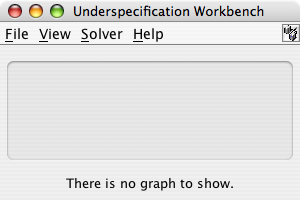
\includegraphics[width=6cm]{ubench-empty.png}
%HEVEA \end{latexonly}
%HEVEA \imgsrc{ubench-empty.png}
\end{quotation}

Now let's have a look at an example. Utool comes with a number of built-in examples, which you can access from Ubench via the File/Open Example menu. So go to this menu, and load the example \verb?holesemantics-14.hs.pl?. This is a Hole Semantics USR for the sentence ``Every man in a restaurant knows a woman with a car'', in the Prolog format used in the Blackburn and Bos textbook \cite{blackburn05:_repres_infer_natur_languag}. Ubench will internally convert this USR into a labelled dominance graph and then draw it as follows:

\begin{quotation}
%HEVEA \begin{latexonly}
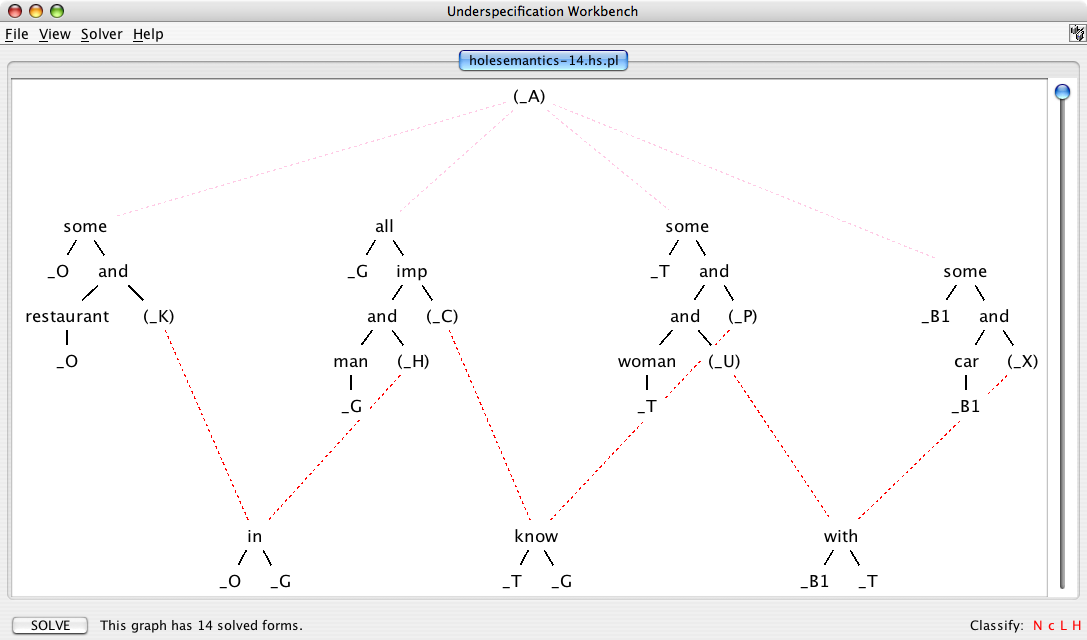
\includegraphics[width=10cm]{ubench-holesem.png}
%HEVEA \end{latexonly}
%HEVEA \imgsrc{ubench-holesem.png}
\end{quotation}

The window displays some interesting information below the dominance graph. In the lower right corner, you will see the letters ``N c L H''. These letters express the membership of the graph in a number of graph classes: If you mouse-over the letters, you will see that the graph is normal, compactifiable, leaf-labelled, and hypernormally connected. (These notions are explained e.g.\ in \citeNP{Koller04}.) This is nice but unsurprising: The translations from Hole Semantics and MRS require the resulting dominance graph to be leaf-labelled and hypernormally connected, because these are formal prerequisites of the correctness of the translations. If the USR hadn't been of this form, Ubench would have refused to translate it and displayed an error message.


\subsubsection{Solving dominance graphs}

In addition, the status bar claims that this dominance graph has 14 \emph{solved forms}. A solved form is an arrangement of the tree fragments (the subgraphs that are connected by solid edges) into a forest, in such a way that if there is a path from node $u$ to node $v$ in the dominance graph (via any kinds of edges), there is still a path from $u$ to $v$ in the solved form. You can look at them by clicking on the ``Solve'' button in the lower left. The result will look as follows:


\begin{quotation}
%HEVEA \begin{latexonly}
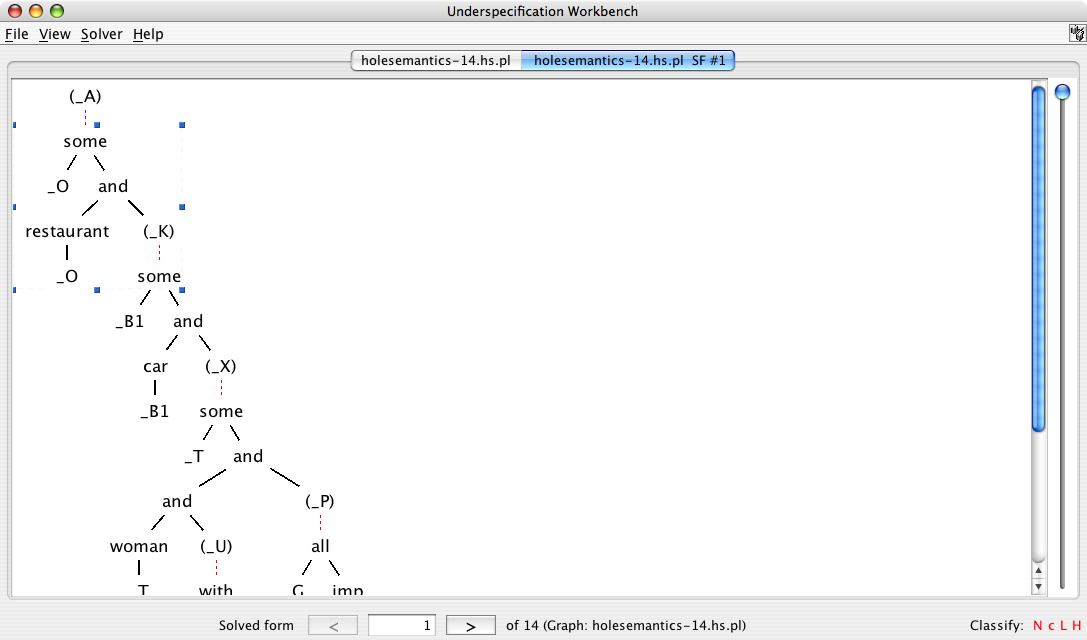
\includegraphics[width=10cm]{ubench-holesem-sf.png}
%HEVEA \end{latexonly}
%HEVEA \imgsrc{ubench-holesem-sf.png}
\end{quotation}

As you can see, Ubench opened a new tab ``holesemantics-14.hs.pl SF \#1'', which displays the first solved form of the graph. In linguistic terms, the solved form represents one of the scope readings, in which the different quantifiers have been assigned one particular scoping. You can see that the solved form may still contain (dotted) dominance edges. But because the original graph was hypernormally connected, you can imagine that they can all be removed and the result is a tree that only consists of tree edges and represents a formula of first-order predicate logic. In technical terms, this is a \emph{configuration} of the original graph; again, see e.g.\ \citeN{Koller04} for details.

Notice that the status bar of a solved form is different than that of an unsolved dominance graph: It now displays the index of the solved form among all solved forms of this graph, and arrows for moving back and forth between the different solved forms. Go ahead and look at some solved forms.



\subsubsection{Exporting graphs and solved forms}

As we have said above, Utool works internally with labelled dominance graphs. It uses modules called \emph{input codecs} to map string representations of USRs in some formalism into labelled dominance graphs. When you opened the example \verb?holesemantics-14.hs.pl? earlier, Ubench recognised that the filename extension \verb?.hs.pl? is associated with the \verb?holesem-comsem? input codec, and used this codec to translate the contents of the file into the graph it displayed for you \cite{KolNieTha03}. Utool is distributed with a number of different input codecs. Some of these (e.g.\ the ones that deal with various concrete syntaxes of dominance graphs) are rather trivial, whereas others (e.g.\ the MRS input codecs) are quite sophisticated and needed to be proved correct \cite{FucKolNieTha04}.

Utool also comes with several \emph{output codecs}, which solve the converse task of computing a string representation for a labelled dominance graph. Let's have a look at these for a moment. Go back to the ``holesemantics-14.hs.pl'' tab, and choose File/Export from the menu. If you open the ``file format'' dropdown menu, you will see the list of output codecs that Ubench is aware of. One thing you can try here is to select the \verb?domgraph-dot? output codec, which exports the current dominance graph in the ``dot'' graph format. Then you can use a graph-drawing tool that can deal with dot files, such as Graphviz, to visualise the graph.

Alternatively, you can make Ubench write all solved forms of the current dominance graph into a file. Choose File/Export Solved Forms from the menu and choose, for instance, the \verb?term-prolog? output codec. This will save all solved forms of the graph as a list of Prolog terms, as they would e.g.\ be computed by the Blackburn and Bos USR solver.

You can display a list of all installed codecs by selecting Help/Show All Codecs in the Ubench menu, or by calling \verb?utool --display-codecs? on the command line. You can also extend Utool/Ubench quite easily by implementing your own codecs. This is described in more detail in Section~\ref{sec:codecs}.



\subsubsection{Redundancy elimination}

Let's finish off the Ubench section of this tutorial with a more advanced operation. Utool is able to modify an underspecified representation in such a way that readings are removed if they are equivalent to some other reading that is still described by the USR. This can be very useful in practice. Consider the following sentence (this is Sentence 1262 from the Rondane Corpus):

\begin{example}
\label{ex:rondane-1262} 
  For travellers going to Finnmark there is a bus service from Oslo to
  Alta through Sweden. 
\end{example}

According to the English Resource Grammar (ERG; \citeNP{Copestake&Flickinger:LKB}), this sentence has got 3960 scope readings. However, this ambiguity only comes from the fact that the ERG analyses proper names as potentially scope-bearing quantifiers, and the only difference between the different readings is the relative scope of these proper-name ``quantifiers''. More generally, we can say that all readings of the sentence are semantically equivalent, and it would be desirable to remove 3959 of these equivalent readings and retain only a single representative. And while the redundancy in this particular example comes only from spurious scope ambiguities between proper names, the problem of reducing the number of logically equivalent reading is not restricted to them and also covers ambiguities between e.g.\ different existential quantifiers or different universal quantifiers.

Utool implements a redundancy elimination algorithm, which will modify a USR in such a way that readings that are semantically equivalent to remaining readings are deleted. It does this without ever enumerating readings, and is thus very efficient \cite{koller06}. At the same time, it is very effective: It reduces the median number of readings on the Rondane Treebank from 55 to 4. Let's try it out.

The first thing you will need is a file that defines equivalences. One such file is distributed with Utool. In order to access it, unpack the Utool Jar file by typing the following command in some directory:

\begin{verbatim}
$ jar xf Utool-3.1.jar
\end{verbatim}

This will create, among many others, a file \verb?erg-examples.xml? in the directory \verb?examples?. This file contains an equivalence definition that is appropriate for the Minimal Recursion Semantics USRs that are computed by the English Resource Grammar \cite{Copestake&Flickinger:LKB}. Remember the pathname of this file for now.

Now go back to Ubench and open the example \verb?rondane-1262.mrs.pl? in Ubench; the filename extension \verb?.mrs.pl? is connected to the \verb?mrs-prolog? input codec, which will read MRS representations in the Prolog format used by the ERG. As you are already familiar with, Ubench will translate the USR into a labelled dominance graph and display it.  Select the entry ``View/Display Chart'' from the menu. This will open a new window that looks as follows:

\begin{quotation}
%HEVEA \begin{latexonly}
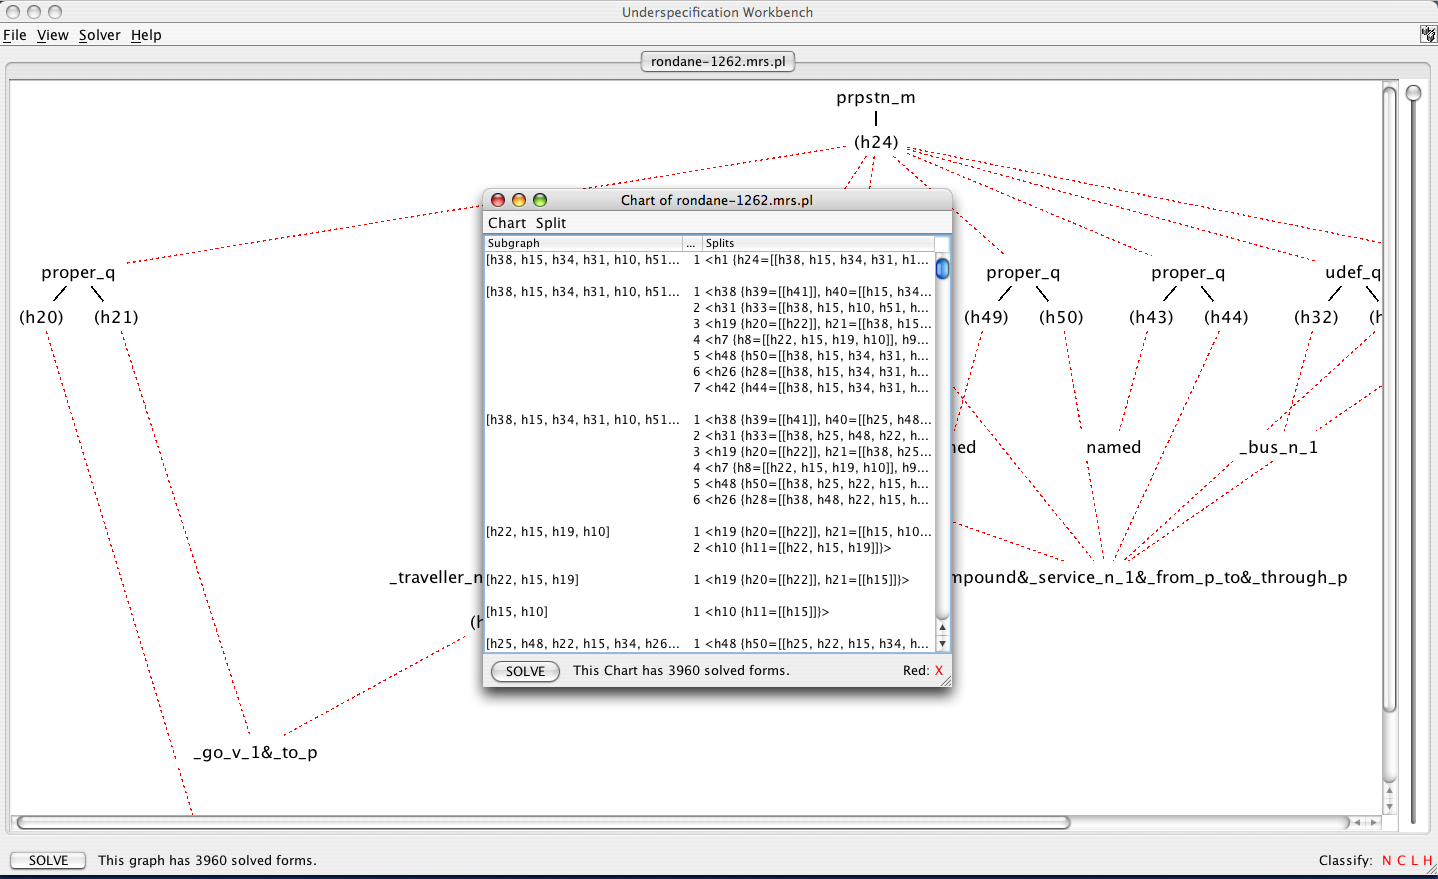
\includegraphics[width=10cm]{ubench-chart.png}
%HEVEA \end{latexonly}
%HEVEA \imgsrc{ubench-chart.png}
\end{quotation}

The new windows displays the \emph{dominance chart} for the dominance graph. The dominance chart is an internal representation of the set of all solved forms that's more explicit and not quite as compact at the dominance graph itself, but still much smaller than the set of solved forms itself (\citeNP{KolTha05b} -- see also Fig.~\ref{fig:chart-vs-solutions}). The chart is interesting in itself, and you can play with it a bit (try clicking on the different entries to highlight subgraphs), but for our current purposes, the main point is that it is on the level of charts that we can do the redundancy elimination. So choose Chart/Reduce Chart from the menu of the chart window, and select the file \verb?erg-examples.xml? that you unpacked from the Jar file earlier. After a moment, most entries will have been deleted from the chart, and the status bar will say that the (smaller) chart represents only a single solved form, rather than the 3960 solved forms that the original chart represented. You can click on the ``solve'' button to display this single solved form. As you can see, Ubench just modified a USR in order to represent a much smaller set of readings, and it did this without computing the individual readings. From our perspective, this ability to eliminate irrelevant readings that were technically predicted by the grammar but not intended in the particular situation is the main reason why underspecification is important.

If you find that you're working with redundancy elimination a lot, and you're using the same equivalence files repeatedly, you can set a global equivalence file in the Solver menu. You can then use it conveniently from every chart window by using the menu entry ``Reduce with global equivalence system''.


\subsection{Running Utool from the command line}

All the functionality that you have just explored from the GUI is also available on the command line. By way of example, let's solve the example file \verb?chain3.clls?, which comes with Utool. This is the \emph{pure chain of length 3}; it is shown in Fig.~\ref{fig:chain3}), and you can also look at it via Ubench. This graph is solvable, and has five solved forms.

In order to enumerate the solved forms of \verb?chain3.clls?, you can call Utool as follows:

\begin{verbatim}
$ utool solve -O term-prolog ex:chain3.clls
f1(a0,f2(a1,f3(a2,a3)))
f1(a0,f3(f2(a1,a2),a3))
f2(f1(a0,a1),f3(a2,a3))
f3(f2(f1(a0,a1),a2),a3)
f3(f1(a0,f2(a1,a2)),a3)
\end{verbatim}


\begin{figure}
%HEVEA \begin{latexonly}
\centering
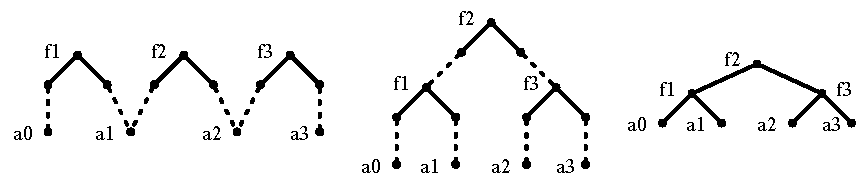
\includegraphics{chain.pdf}
%HEVEA \end{latexonly}
%HEVEA \imgsrc{chain.png}
\caption{The chain of length 3 (left), along with one of its five
solved forms (middle) and one of its configurations (right).
\label{fig:chain3}}
\end{figure}


As you can see, the Utool command line consists of four parts:
\begin{itemize}
\item \verb?utool? (or \verb?java -jar Utool-3.1.jar?): This instructs
Java to load the Jar file and run its main class. You can pass further
arguments to the Java VM by putting them before the \verb?-jar?
option.

\item \verb?solve?: This is the \emph{command} that Utool should execute. In the example, we have run the \verb?solve? command, which enumerates all solved forms of the USR and prints them. There are six other commands --
\verb?solvable?, \verb?convert?, \verb?classify?,
\verb?display?, \verb?server?, and \verb?help? -- which perform
different tasks. They are described in detail in Section~\ref{sec:operations}.

\item \verb?-O term-prolog?: After the command, you can specify \emph{options}. The option \verb?-O term-prolog? (or, equivalently, \verb?--output-codec term-prolog?) specifies that the \verb?solve? command should encode the solved forms using the \verb?term-prolog? output codec. You could have specified the input codec with the \verb?-I? or \verb?--input-codec? option, but Utool already inferred that it should use the input codec \verb?domcon-oz? from the filename extension \verb?.clls?.

\item \verb?ex:chain3.clls?: Finally, you can specify where the input USR should come from. In this example, we have used \verb?ex:chain3.clls?. This tells Utool that it should look inside its Jar file for a resource with the name \verb?examples/chain3.clls? and read the USR from there. Alternatively, you can specify an ordinary filename here, and Utool will read the input USR from your file system. You can also pass a hyphen (\verb?-?) for this argument to make Utool read its input from standard input.
\end{itemize}


Some USRs have a lot of readings, and you either don't want to see them all, or it takes too long to enumerate them, but are still curious about how many readings the USR has. This is what the \verb?solvable? command is for. You run it as follows:

\begin{verbatim}
$ utool solvable -s ex:thatwould.clls
The input graph is normal.
The input graph is not compact, but I will compactify it for you.

Solving graph ... it is solvable.
Splits in chart: 650
Time to build chart: 105 ms
Number of solved forms: 64764
\end{verbatim}

As you can see, we have now instructed Utool to run the \verb?solvable? command on the input USR \verb?ex:thatwould.clls?. In addition, we have specified the \verb?-s? (or \verb?--display-statistics?) option to get more informative output. Notice that we didn't have to specify an output codec, because \verb?solvable? doesn't output USRs or readings.

Utool has computed a dominance chart with 650 entries and established that this chart represents a set of 64764 solved forms. However, it has not actually computed the solved forms themselves. (This is what \verb?solve? would have done after computing the chart.) It has also set an \emph{exit code} of 1 because the graph is solvable (has solved forms), so if you are using a bash shell, you can do the following immediately after the utool call:

\begin{verbatim}
$ echo $?
1
\end{verbatim}

If you want to give your computer a challenge, we encourage you to run \verb?solvable? on the input \verb?ex:rondane-650.mrs.pl?, an MRS USR representing more than two trillion readings. You will have to increase Java's memory limit by passing it the option \verb?-Xmx512m? to avoid ``out of memory'' errors.


Two further Utool commands are \verb?convert? and \verb?classify?, which allow you to convert USRs into other formalisms (comparable to opening a USR and then exporting it using a different codec in Ubench) and to determine their membership in various graph classes (a more sophisticated version of Ubench's ``N C L H'' display in the status bar). We will not cover these commands in this tutorial. However, it is worth pointing out that you can always get help on the command-line usage of Ubench using the \verb?help? command:

\begin{verbatim}
$ utool help
\end{verbatim}

will display an overview of possible commands, whereas

\begin{verbatim}
$ utool help solve
\end{verbatim}

will display help on how to use the \verb?solve? command (and similarly for the other commands).




\subsection{The Utool Server} 

The third way of running Utool is in a server mode. In server mode, Utool
keeps running indefinitely; it accepts commands via a socket, executes
these commands, and sends the results back through the socket. You can
start Utool in server mode from Ubench by clicking on the server icon in the top right corner, or from the command line as follows:

\begin{verbatim}
$ utool server
\end{verbatim}
%$

This will open a socket on port 2802 of your machine and listen to
commands sent to this port. If you have Perl installed on your
system, you can test the Utool Server using the demo client we have
included in the distribution. Keep the Utool server process
running, change to the directory where you unpacked the Jar earlier, and execute the following command:

\begin{verbatim}
$ perl tools/client/utool-client.pl solve -I domcon-oz -O term-prolog \
         examples/chain3.clls
f1(a0,f2(a1,f3(a2,a3)))
f1(a0,f3(f2(a1,a2),a3))
f2(f1(a0,a1),f3(a2,a3))
f3(f2(f1(a0,a1),a2),a3)
f3(f1(a0,f2(a1,a2)),a3)
\end{verbatim}

The server supports exactly the same commands as the command-line
version (except that you can't use it to start another
server). However, it has the advantage that you need to run only a
single process to execute any number of commands, whereas you must
start a new Java process for each new command when you use the
command-line tool. This saves runtime if you need to run a large
number of successive commands, such as when classifying all USRs in a
corpus: You don't have the overhead for starting Java, and the
programme will also become faster over time because the Java system
has the opportunity to just-in-time compile the Java bytecode.



\ignore{






\subsection{Checking whether an USR is solvable}

First of all, let's use Utool to determine whether a given dominance
graph is solvable. ``Solvable'' means that it is possible to configure
the fragments of the graph (i.e.\ those subgraphs which are connected
by solid ``tree'' edges) into a forest while realising the (dotted)
dominance edges as reachability in the tree. Such a forest-shaped
arrangement of a dominance graph is called a \emph{solved form} (see
Fig.~\ref{fig:chain3}). Many solvable graphs also have
\emph{configurations}, i.e.\ trees that consist only of the labelled
nodes in the dominance graph, connected by tree edges. All this is
defined in detail e.g.\ in \cite{Koller04}.

We will do this for the graph specified in the file
\url{examples/chain-3.clls} (shown 

The Utool command for checking solvability is called
\verb?solvable?. Thus you can check the example graph for solvability
as follows:

\begin{verbatim}
$ utool solvable -s examples/chain-3.clls
The input graph is normal.
The input graph is compact.

Solving graph ... it is solvable.
Splits in chart: 10
Time to build chart: 60 ms
Number of solved forms: 5
\end{verbatim}
%$

The output states that the graph is solvable and has five solved
forms. It also contains some information about the input graph (it is
normal and compact), the chart data structure computed by the solver
(it contains ten splits), and the time it took to compute the
chart. In addition, the program terminated with an exit code of 1 to
signal that the graph was indeed solvable. If you ran Utool from a
bash shell, you can display this exit code with the command
``\verb!echo $?!''. %$

As you can see, the Utool command line consists of four parts:
\begin{itemize}
\item \verb?utool? (or \verb?java -jar Utool-3.1.jar?): This instructs
Java to load the Jar file and run its main class. You can pass further
arguments to the Java VM by putting them before the \verb?-jar?
option.
\item \verb?solvable?: Most of the time, a call to Utool will contain
exactly one \emph{command}. There are seven commands --
\verb?solvable?, \verb?solve?, \verb?convert?, \verb?classify?,
\verb?display?, \verb?server?, and \verb?help? -- which perform
different tasks. We will walk you through all seven commands here, and
then describe them in more detail in Section~\ref{sec:operations}.
\item \verb?-s?: After the command, you can specify \emph{options}. In
this case, we selected one option (\verb?-s? or
\verb?--display-statistics?), which was responsible for printing all
the output from the example run above. We could have left the option
away; then the Utool run would have done exactly the same, and
returned the same exit code, but it wouldn't have printed these
informational messages.
\item \verb?examples/chain-3.clls?: This is the name
of the file from which the dominance graph should be read. The file
can contain a direct specification of a dominance graph (as in this
case), or it can contain an USR of some other underspecification
formalism which is then translated to a dominance graph
automatically.
\end{itemize}



\subsection{Enumerating solutions}

Now that we know that the dominance graph is solvable, let's have
Utool show us the five solved forms that it claimed exist. We do this
using the \verb?solve?  command, like so:

\begin{verbatim}
$ utool solve -O term-prolog examples/chain3.clls
f1(a0,f2(a1,f3(a2,a3)))
f1(a0,f3(f2(a1,a2),a3))
f2(f1(a0,a1),f3(a2,a3))
f3(f2(f1(a0,a1),a2),a3)
f3(f1(a0,f2(a1,a2)),a3)
\end{verbatim}
%$

The five solved forms of the graph are displayed as terms in Prolog
syntax: Utool transforms each solved form into a \emph{configuration}
by identifying roots and holes as shown in Fig.~\ref{fig:chain3}, and
then prints the resulting trees as ground terms. You may want to
convince yourself at this point that the graph indeed has exactly five
solved forms, and that the five terms shown above are such term
representations of the configurations.

We had to use a new command-line option in the \verb?solve? command:
\verb?-O term-prolog? (which is shorthand for
\verb?--output-codec term-prolog?). Once Utool has computed a solved
form, it needs to know how it should translate this solved form into a
string representation. This translation is handled by an \emph{output
codec}. A number of output codecs are distributed with Utool; you can
also implement your own output codec if you like. In the example, we
used the \verb?term-prolog? output codec, which maps solved forms into
configurations and these configurations into Prolog terms as explained
above.

Speaking of codecs: There are also \emph{input codecs}, which map from
a string representation of an USR into a dominance graph. In the
example, Utool read the string representation from the file with the
specified name (\url{chain3.clls}) and passed it to an input codec to
obtain a dominance graph from it. In this case, we didn't have to
specify the input codec explicity, because Utool knows that the
filename extension \verb?.clls? is associated with the
\verb?domcon-oz? input codec, and used this codec automatically. We
could also have specified the input codec explicitly using the
\verb?-I domcon-oz? or \verb?--input-codec domcon-oz? option. Codecs
can be much more powerful than the ones mentioned here, and are
described in depth in Section~\ref{sec:codecs}.

 
\subsection{Converting and classifying USRs}

Utool works with labelled dominance graphs internally; input codecs
are used to translate from other formalisms into labelled dominance
graphs, and output codecs are used to translate from labelled
dominance graphs into other formalisms. These translations can be
non-trivial, and we have defined and proven them correct in several
research papers \cite{KolNieTha03,mrs-dom}.

A special case is if you make Utool read a USR in some formalism,
which it translates into a labelled dominance graph, and then output
this same labelled dominance graph using a different output
codec. What this does is essentially to convert a USR into an
equivalent USR in some other formalism. This allows you to use our
theoretical groundwork on formal translations between
underspecification formalisms in a convenient way, and can be useful
in certain situations.

Let's look at an example again. The file
\url{examples/rondane-1.mrs.pl} is an USR in the
Minimal Recursion Semantics formalism \cite{CopFliSag97}. This MRS is
computed by the English Resource Grammar
\cite{Copestake&Flickinger:LKB} for the first sentence in the Rondane
Treebank, which is distributed with the ERG. Its filename extension is
\verb?.mrs.pl?, which is associated with the \verb?mrs-prolog? input
codec. Now let's convert this MRS into a labelled dominance graph in
Oz syntax (output codec \verb?domcon-oz?).

\begin{verbatim}
$ utool convert examples/rondane-1.mrs.pl -O domcon-oz
%% autogenerated by Utool 3.1 (see www.coli.uni-sb.de/projects/chorus/utool for details)
[label(h54 named) label(h51 proper_q(h52 h53)) label(h45 '_of_p&_part_n&_and_c'(
h43 h47)) label(h47 '_western_a') label(h43 '_eastern_a') label(h40 '_the_q'(h42
 h41)) label(h36 '_between_p&_route_n&_main_a') label(h33 '_the_q'(h35 h34)) lab
el(h25 '_of_p_sel&card&part_of') label(h27 def_explicit_q(h28 h29)) label(h23 '_
once_a'(h24)) label(h21 '_be_v_id') label(h10 '_valley_n&compound&_and_c'(h8 h12
)) label(h19 named) label(h16 proper_q(h17 h18)) label(h12 '_historic_a') label(
h8 '_well+known_a') label(h4 '_the_q'(h7 h5)) label(h1 prpstn_m(h3)) dom(h52 h54
) dom(h42 h45) dom(h35 h36) dom(h28 h25) dom(h24 h21) dom(h17 h19) dom(h7 h10) d
om(h3 h23) dom(h3 h33) dom(h3 h16) dom(h3 h27) dom(h3 h40) dom(h3 h51) dom(h3 h4
) dom(h34 h25) dom(h18 h10) dom(h29 h21) dom(h41 h36) dom(h53 h45) dom(h5 h21)]
\end{verbatim}
%$


In addition, Utool can check for you whether the labelled dominance
graph it works with belongs to one of a number of important classes
using the \verb?classify? command, like so:

\begin{verbatim}
$ utool classify -s examples/rondane-1.mrs.pl
The input graph is normal.
The input graph is not compact, but I will compactify it for you.
The graph is hypernormally connected.
The graph is leaf-labelled.
\end{verbatim}
%$

Among other things, Utool just told us that the graph is
\emph{hypernormally connected} and \emph{leaf-labelled}
\cite{KolNieTha03}. This is very important because USRs written in MRS
or Hole Semantics can only be correctly encoded into a labelled
dominance graph if the resulting graph has these two properties; the
technical reason for this is that we can guarantee that every solved
form has a configuration only for such graphs. We hypothesise that all
correct USRs that are currently produced by large-scale grammars are
indeed hypernormally connected and leaf-labelled; using the
\verb?classify? command, we can quickly go through a large number of
USRs from a corpus and test this hypothesis \cite{FliKolTha05}.

One final note is that if you call Utool from a script that does such
batch processing, you can conveniently retrieve the classification by
looking at the exit code of the Utool process. For instance, a bash
shell makes the exit code of the previous process accessible to you in
the \verb!$?! shell variable, so you get the following result:

\begin{verbatim}
$ echo $?
59
\end{verbatim}
%$

The exit code $59 = 32 + 16 + 8 + 2 + 1$ indicates that the graph is
leaf-labelled, hypernormally connected, compactifiable, normal, and
weakly normal, but not compact. These exit codes are documented in
Section~\ref{sec:op-classify} below. 



\subsection{The Underspecification Workbench} 

Utool comes with a graphical user interface (Ubench, the
Underspecification Workbench) which will display labelled dominance
graphs and their solved forms and give you access to all the
functionality that is also available from the command-line tool.

You can start Ubench as follows:
\begin{verbatim}
$ utool display
\end{verbatim}
%$

\begin{figure}
\begin{center}
%HEVEA \imgsrc{ubench.png}
%HEVEA \begin{latexonly}
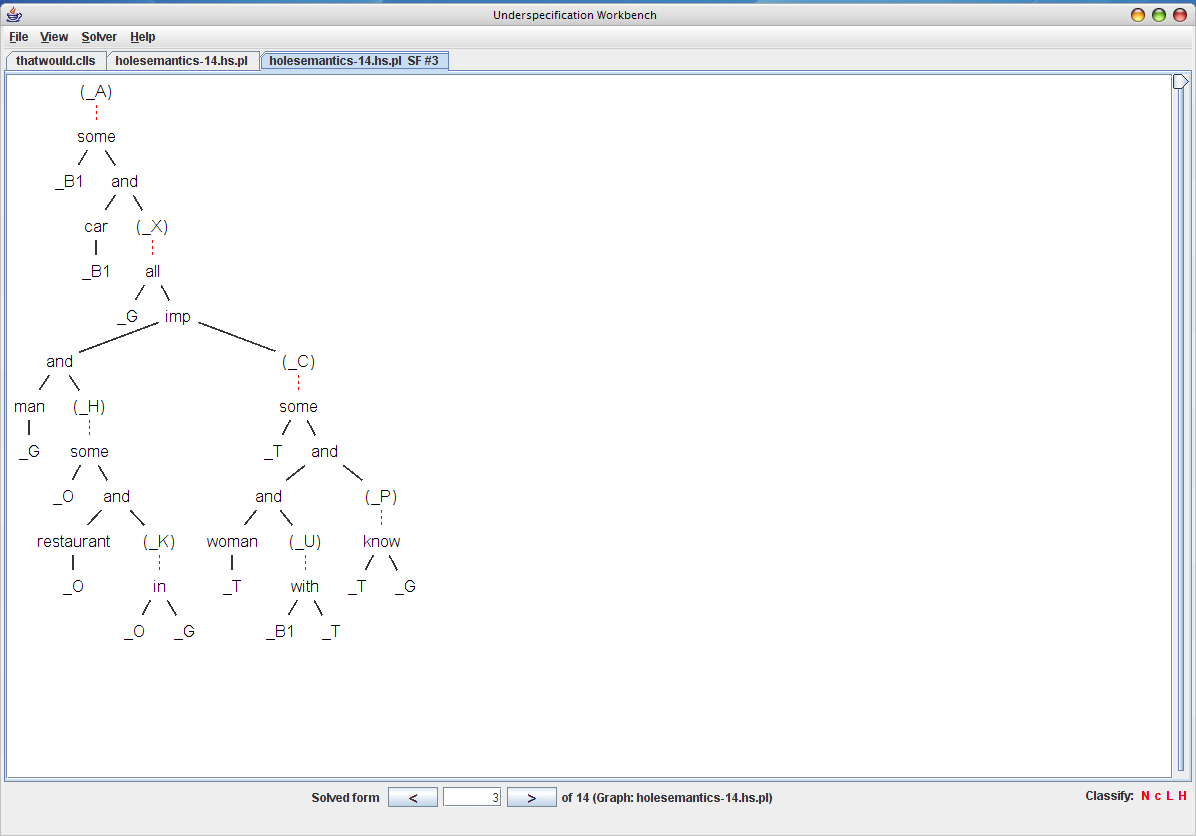
\includegraphics[width=0.8\textwidth]{ubench.png}
%HEVEA \end{latexonly}
\end{center}
\caption{The Underspecification Workbench. \label{fig:ubench}}
\end{figure}


This will bring up the main Ubench window (see
Fig.~\ref{fig:ubench}). At this point, it displays just a menu and an
empty content pane, but you can use the File/Open menu to load
USRs. Alternatively, you can pass the name of an USR file to Ubench
directly as follows:

\begin{verbatim}
$ utool display examples/rondane-1.mrs.pl
\end{verbatim}
%$

This will load the given USR and display it immediately. Notice that
Ubench automatically classifies new USRs it loads, and displays the
results in the lower right corner of the window. It also solves the
USR and displays the number of solved forms. You can then click on the
``Solve'' button to display the first solved form, and then cycle
through the other solved forms from there. In addition, Ubench is able
to export an USR using another output codec (through the File/Export
menu), or export the graph as it is currently drawn as a PDF file
(through the File/Export as PDF menu).

}



%%% Local Variables: 
%%% mode: latex
%%% TeX-master: "0"
%%% TeX-command-default: "LaTeX"
%%% End: 

\section{Using Utool}  \label{sec:operations}

In the current release, Utool supports six commands: \verb?solve?,
\verb?solvable?, \verb?classify?, \verb?convert?, \verb?server?,
\verb?display?. Each of these commands can be used from the
command-line or in the Utool Server (but running the \verb?server?
command in the Utool Server doesn't do anything). In addition, Utool
supports several auxiliary pseudo-commands, which display help
information. 

In this section, we describe these commands in some detail.


\subsection{Command-line interface}
When Utool is run from the command-line, it executes the single
command you specify on the command line and then exits. For instance,
the following call executes one \verb?solvable? command and outputs
some information about it:

\begin{verbatim}
$ utool solvable -s chain-3.clls
\end{verbatim}
% $

Commands typically require \emph{arguments} (in the example, the
filename \verb?chain-3.clls? of the USR that we want to solve), and
accept certain \emph{options} (here, the \verb?-s? option, which
instructs Utool to display statistical information). These arguments
and options are written after the command on the command line.


\subsection{Server mode} \label{sec:operations-server}

Alternatively, you can run Utool in server mode. In this mode, it will
not execute any commands at first. Instead, it will accept network
connections on a specific socket. Each time it is sent a command on
this socket, it will execute this command, send the results back over
the socket, and then close the socket. But the same Utool process
keeps running and can execute many commands during its lifetime. 

You start Utool in server mode by making Utool execute the
\verb?server? command:

\begin{verbatim}
$ utool server
\end{verbatim}
%$

The server doesn't output anything on the console on which you started
it -- unless you specified the \verb?--logging? command-line option
and no name for the logfile, in which case it will write some
information to standard error. 

By default, the server will listen for socket connections on port
2802, but the port can be specified using the \verb?--port?
option. The protocol for communicating with the server is as follows:


\begin{enumerate}
\item The client sends a command in an XML element of the following
form: 
\begin{verbatim}
<utool cmd="..." (more options)>
  (arguments of the command)
</utool>
\end{verbatim}

The command, options, and arguments in this XML element correspond to
the command, options, and arguments of a single run of the
command-line tool.

\item The client shuts down the half of the socket that is responsible
for sending data to the server (i.e.\ the ``output'' direction). Many
socket libraries (e.g.\ the standard libraries for C and Perl) offer a
\verb?shutdown? function for this purpose. Notice that \verb?shutdown?
is different from \verb?close? because it only closes one direction of
the socket; you can't close the socket yet because you still need to
receive the response from the server.

\item Once the client-to-server socket is shut down, the Utool Server
processes the command.

\item If the command is executed successfully, the server will respond
with a message of the following form:

\begin{verbatim}
<result .... />
\end{verbatim}

The particular attributes of this element depend on the command, and
are described below. If an error occurred, the response will be a
message of the following form instead:

\begin{verbatim}
<error code="..." explanation="..." />
\end{verbatim}

Here the ``code'' attribute will be a numeric error code, and the
``explanation'' attribute will be a plain-text explanation of the
error that occurred.

\item The server closes the socket.
\end{enumerate}


If you just use Utool for a single call or experimentation, the
command-line mode will typically be easier to use. However, if you
need to process many Utool commands from a programme, it can be
dramatically more efficient to keep a single Utool Server process
running and send the commands to the server (see
Section~\ref{sec:practice-some-practical-tips}). We present a demo
client for the Utool Server in Section~\ref{sec:practice-client}.


\subsection{Passing USRs}

Most commands require the user to specify an USR that should be
processed.

In command-line mode, you pass a specification of the USR as a
command-line argument. Most input codecs interpret this specification
string as the filename from which the USR should be read; in the
example above, we used the file name \verb?chain-3.clls?. However, it
is up to the input codec to decide how the argument string should be
interpreted; the \verb?chain? codec, for example, interprets the
string as the chain length and not as a filename.

In server mode, you can't pass a filename because the server may run
on a different machine than the client and may not have access to its
filesystem. Instead, you pass the USR directly as an attribute of a
\verb?usr? element that is embedded into the \verb?utool? element,
like so:

\begin{verbatim}
<utool cmd="solvable">
  <usr codec="domcon-oz" string="[label(x f(y)) ...]" />
</utool>
\end{verbatim}

Notice that the attribute values must be valid XML attribute
strings. This means that you must replace special characters by
their respective character entities (see also
Section~\ref{sec:practice} for tips on this).


\subsection{Exit codes}

Each execution of a Utool command returns an \emph{exit code}. The
command-line version of Utool will return this as the programme exit
code, which you can access e.g.\ in the \texttt{\$?} variable in a
Bash shell. The server version will return the exit code in the
\verb?code? attribute in the responses for many commands (and always
when it reports an error).

Exit codes are numbers between 0 and 255. They are split up into
ranges with different meanings as follows:

\begin{tabular}{l|l}
exit codes & meaning \\\hline
0 -- 127 & command was executed successfully \\
128 -- 191 & an error occurred in the main programme \\
192 -- 223 & an error occurred in the input codec \\
224 -- 255 & an error occurred in the output codec
\end{tabular}

The exit codes for successful termination of a command are documented
with the commands below. Among the codec error codes, the code 192 is
special because it always signifies a parsing error in the input
codec. The codes between 193 and 223 denote \emph{semantic errors} in
the input codec; they and all output codec error codes are documented
with the codecs in Section~\ref{sec:codecs}. The error codes for the
main programme are as follows:

\begin{tabular}{l|l}
exit code & meaning \\\hline
128 & file I/O error \\
129 & network I/O error \\
130 & Ubench encountered an error while laying out a graph \\

140 & error while configuring an (XML) parser \\
141 & the command you specified was not recognised \\
142 & error while registering a codec \\

150 & you didn't specify a USR, but the command requires one \\
151 & you didn't specify an input codec, and Utool cannot guess it \\
152 & there is no input codec of the name you specified \\
153 & the input graph is not weakly normal or not compactifiable \\

160 & you didn't specify an output codec, and Utool cannot guess it \\
161 & there is no output codec of the name you specified \\

170 & error while parsing an equivalence specification
\end{tabular}




\subsection{The commands supported by Utool}

We will now go through the seven main commands and describe what each
command does and what options it takes.


\subsubsection{Solvable}

This command converts the input USR into a dominance graph and checks
whether this graph is solvable, i.e.\ has any
solutions. Linguistically, this corresponds to checking whether the
sentence has any readings (ideally, it should!).

Solvability is determined by computing a dominance chart as described
in \cite{KolTha05b}. This is typically much more efficient than
actually \emph{solving} the graph, i.e.\ enumerating its solved forms,
because the chart is exponentially smaller than the set of all solved
forms. This command only makes a yes/no decision about solvability and
thus doesn't have to enumerate all the solved forms. If you want them,
see the ``solve'' command below.


\paragraph{Result.}
In command-line mode, the Utool process will terminate with an exit
code of 1 if the graph was solvable. It will terminate with an exit
code of 0 if it wasn't. 

In server mode, Utool will send a reply of the following form:
\begin{verbatim}
<result solvable='true' fragments='7' count='5' chartsize='10' time='30' />
\end{verbatim}

The \verb?solvable? attribute contains the string \verb?true? if the
graph was solvable, and \verb?false? otherwise. The other attributes
contain statistical information: the number of fragments of the graph,
the number of solved forms, the number of splits in the chart, and the
time in milliseconds it took to compute the chart.


\paragraph{Options.}
The \verb?solvable? command can take the following options:
\begin{itemize}
\item \textbf{input-codec:} You can specify an input codec for this
command. If you don't do this, the command-line version (but not the
server) will try to guess the appropriate input codec from the
filename extension if possible.

In command-line mode, specify the input codec with the option
\verb?--input-codec <codecname>? or \verb?-I <codecname>?. In server
mode, specify it as the \verb?codec? attribute of the \verb?usr?
element.

\item \textbf{display-statistics:} You can make Utool display more detailed
statistics when you call it on the command-line by passing the
\verb?--display-statistics? or \verb?-s? option. All such statistics
information will be written to standard error.
\end{itemize}




\subsubsection{Solve}

This command converts the input USR into a dominance graph, computes
the solved forms of this graph, and outputs them using the given
output codec. It computes a dominance chart, and if the graph was
solvable, proceeds to enumerate all solved forms.


\paragraph{Result.}
In command-line mode, Utool will output all solved forms. By default,
it will write them to standard output, but there is a command-line
option for redirecting them into a file. This command will always
terminate with an exit code of 0 if no errors occurred.

In server mode, Utool will send a reply of the following form:
\begin{verbatim}
<result solvable='true' fragments='7' count='5' chartsize='10'
        time-chart='30' time-extraction='100'>
  <solution string='....' />
  <solution string='....' />
</result>
\end{verbatim}

The attributes of the \verb?result? element are as for the
\verb?solvable? command, except that the runtime is now reported
separately for computing the chart and for enumerating (extracting)
the solved forms. The solutions are returned in attributes of
\verb?solution? elements below the \verb?result? element. Notice that
you may need to resolve XML character entities that were used in the
attribute value strings.

\paragraph{Options.}
The \verb?solve? command can take the following options:
\begin{itemize}
\item \textbf{input-codec:} see \verb?solvable?
\item \textbf{output-codec:} You can specify the output codec which
should be used to encode the solved forms. If you don't specify the
output codec explicitly, the command-line tool will first try to guess
the output codec from the output filename if you specify one. If this
doesn't work, it will try to use the output codec with the same name
as the input codec, if it exists. The server will not make such
guesses and expects you to specify the codec explicitly in any case.

In command-line mode, specify the output codec with the option
\verb?--output-codec <codecname>? or \verb?-O <codecname>?. In server
mode, specify it by passing the codec name as the \verb?output-codec?
attribute of the main \verb?utool? element.

\item \textbf{output:} By default, the command-line tool will write
the encoded solved forms to standard output. You can override this by
specifying an output file with the option \verb?--output <filename>?
or \verb?-o <filename>?. This option is not applicable in server mode
because it doesn't write into files anyway.

\item \textbf{no-output:} You can instruct Utool not to output the
actual solved forms by specifying the ``no-output'' option. Utool will
still \emph{compute} all solved forms in this case, it will simply not
\emph{output} them. This can be useful for runtime
measurements. Specify the option \verb?--no-output? or \verb?-n? on
the command line. In server mode, you get this effect if you simply
don't specify any output codec in the \verb?utool? element.

\item \textbf{display-statistics:} see \verb?solvable? 
\end{itemize}






\subsubsection{Convert}

This command reads a USR and outputs it again. The point about this
operation is that the input and output codecs may be different. This
means that you can use it to convert USRs from one underspecification
formalism to another (to the extent that this is supported by theory).

\paragraph{Result.}
In command-line mode, Utool will output the USR using the specified
output codec. By default, it will write it to standard output, but you
can again redirect the output to a file. The command always returns an
exit code 0 on successful completion.

In server mode, Utool will send a reply of the following form:
\begin{verbatim}
<result usr='....' />
\end{verbatim}

The string in the \verb?usr? attribute is the converted USR. Remember
that you may need to resolve XML character entities that were used in
the attribute value strings.

\paragraph{Options.}
The \verb?convert? command can take the following options:
\begin{itemize}
\item \textbf{input-codec:} see \verb?solvable? 
\item \textbf{output-codec:} see \verb?solve? 
\item \textbf{output:} see \verb?solve?
\item \textbf{no-output:} see \verb?solve?
\item \textbf{display-statistics:} see \verb?solvable?
\end{itemize}




\subsubsection{Classify} \label{sec:op-classify}

The \verb?classify? command checks whether a dominance graph belongs
to certain particularly well-behaved classes. It currently
distinguishes the following classes:

\begin{itemize}
\item \emph{weakly normal}: A dominance graph is weakly normal
\cite{bodirsky-weakly-normal-constraints} if the tree edges form a
forest and all dominance edges go into roots.
\item \emph{normal}: A weakly normal dominance graph is normal
\cite{Althaus-J.Algo.} if all dominance edges also start in
(unlabelled) holes.
\item \emph{compact}: A weakly normal dominance graph is compact if
all fragments have depth zero or one, i.e.\ no node has both incoming
and outgoing tree edges.
\item \emph{compactifiable:} Many weakly normal graphs that are not
compact can nevertheless be made compact by removing internal nodes
and labelled leaves of fragments, and adding tree edges from the roots
to the holes. In particular, all normal graphs are compactifiable. If
a graph is compactifiable, it is guaranteed that there is a one-to-one
correspondence between the solved forms of the compactified graph and
the solved forms of the original graph.
\item \emph{hypernormally connected:} A normal graph is hypernormally
connected \cite{KolNieTha03,Koller04} if any pair of nodes is
connected by a simple hypernormal path, where a hypernormal path is an
undirected path that uses no two dominance edges that are adjacent to
the same hole. This graph class is a bit abstract, but immensely
useful because these graphs (a) have a lot of nice structural
properties, and (b) we believe that all graphs that are currently used
in underspecification are or should be hypernormally connected
\cite{FucKolNieTha04}. Because of (a), the translations of MRS and
Hole Semantics into dominance graphs only work for USRs that translate
into hypernormally connected graphs.
\item \emph{leaf-labelled:} A weakly normal graph is leaf-labelled
\cite{KolNieTha03} if every (unlabelled) hole has an outgoing
dominance edge. If a graph is both hypernormally connected and
leaf-labelled, each of its solved forms has a configuration.
\end{itemize}


\paragraph{Result.}
The classes to which a graph belongs are encoded as the bit-wise OR of
the following values:

\begin{center}
\begin{tabular}{l|l}
class & bit value \\ \hline
weakly normal & 1 \\
normal & 2 \\
compact & 4 \\
compactifiable & 8 \\
hypernormally connected & 16 \\
leaf-labelled & 32
\end{tabular}
\end{center}

The command-line tool will return this value as its exit code upon
successful completion.

The Utool Server will return a message of the following form:
\begin{verbatim}
<result code='63' weaklynormal='true' normal='true'
        compact='true' compactifiable='true'
        hypernormallyconnected='true' leaflabelled='true' />
\end{verbatim}

Here \verb?code? is the exit code described above, and the other
attributes are either \verb?true? or \verb?false?.


\paragraph{Options.}
The \verb?classify? command can take the following options:
\begin{itemize}
\item \textbf{input-codec:} see \verb?solvable? 
\item \textbf{display-statistics:} see \verb?solvable?
\end{itemize}



\subsubsection{Server}

The \verb?server? command starts a new Utool Server. By default, this
server listens to new connections on port 2802, but you can specify a
different port using the \verb?--port? option. This command is ignored
if Utool is already running in server mode; it can only be run from
the command line.

\paragraph{Result.} This command doesn't terminate by itself; you have
to shut down the server process by hand.

\paragraph{Options.} The \verb?server? command can take the following
options:

\begin{itemize}
\item \textbf{port:} By default, the server will listen on a socket on port
2802. You can specify a different port using the option
\verb?--port <number>? (or \verb?-p <number>?), where \verb?<number>?
is the port number you want.

\item \textbf{logging:} Using this option, you can make the server log
information about incoming commands and its responses. If you specify
the option \verb?--logging? (or \verb?-l?) by itself, the log messages
will be written to standard error. Alternatively, you can log the
messages into a file by specifying the filename:
\verb?--logging <filename>? or \verb?-l <filename>?.
\end{itemize}




\subsubsection{Display}

The \verb?display? command instructs Utool to display the input USR in
the Underspecification Workbench (Ubench). If the Utool process has
opened a Ubench window before, it will display the USR in a new tab of
the same window; otherwise it will open a new Ubench window first.

Unlike the previous commands which accept USRs as input, the input USR
argument is \emph{optional} in the \verb?display? command. This means
that you may specify an input USR (in which case it is displayed right
away), or you can call \verb?display? without arguments. In this case,
an empty Ubench window is displayed; you can still open USRs from the
File/Open menu or by sending further \verb?display? commands to the
Utool Server.

Ubench offers a large subset of Utool's functionality from within a
convenient GUI. However, some functions are not accessible from Ubench
-- for example, Ubench doesn't support codec options yet, and you
can't use it to write all solved forms of a USR to a file in one
go. We plan to make this functionality available in Version 3.1.


\paragraph{Result.} This command doesn't terminate by itself; you have
to quit Ubench by choosing the File/Quit menu entry.

\paragraph{Options.} The \verb?display? command can take the following
options:

\begin{itemize}
\item \textbf{input-codec:} see \verb?solvable? 
\end{itemize}




\subsection{Pseudo-commands}

In addition to the six main commands, the command-line version of
Utool will accept a number of ``pseudo-commands'', which display help
information. If you call Utool with a pseudo-command, it executes the
pseudo-command and terminates immediately. You cannot specify both a
command and a pseudo-command at the same time.

The following pseudo-commands exist:

\begin{itemize}
\item \verb?help [command]?: If you specify a command, this will
display a brief help message for that command. Otherwise, it will
display an overview over the possible commands.
\item \verb?--version?: Displays the version of Utool.
\item \verb?--display-codecs? or \verb?-d?: Displays the installed
codecs.
\item \verb?--help-options?: Displays an overview over some frequently
used options.
\end{itemize}




\subsection{Advanced options}

\subsubsection{Redundancy Elimination} \label{sec:redund-elim}

\cite{koller06,koller06:_towar}




\subsection{Options overview}

We conclude this section with an overview over all options.

\newcommand{\optiondesc}[4]{\item #1 \\ (Server mode: #2) \\
(applies to: #3) \\ \strut\\ #4}

\begin{itemize}
\optiondesc
{\texttt{--input-codec <codecname>} or \texttt{-I <codecname>}}
{\texttt{codec} attribute of the \texttt{usr} elements}
{\texttt{solvable}, \texttt{solve}, \texttt{classify}, \texttt{convert}}
{Specify the input codec.}

\optiondesc{\texttt{--input-codec-options <options>}}
{\texttt{codec-options} attribute of the \texttt{usr} elements}
{\texttt{solvable}, \texttt{solve}, \texttt{classify}, \texttt{convert}}
{If the selected input codec accepts options, use this option to
specify them.}

\optiondesc{\texttt{--output-codec <codecname>} or \texttt{-O <codecname>}}
{\texttt{output-codec} attribute of the \texttt{utool} element}
{\texttt{solve}, \texttt{convert}}
{Specify the output codec.}

\optiondesc{\texttt{--output-codec-options <options>}}
{\texttt{output-codec-options} attribute of the \texttt{utool} element}
{\texttt{solve}, \texttt{convert}}
{If the selected output codec accepts options, use this option to
specify them.}

\optiondesc{\texttt{--no-output} or \texttt{-n}}
{assumes this option if no output codec is specified}
{\texttt{solve}, \texttt{convert}}
{Compute the output, but don't display it (useful for runtime
measurements). If you specify this option, you don't need to specify
the output codec (and if you do, it is ignored). }

\optiondesc{\texttt{--output <filename>} or \texttt{-o <filename>}}
{not applicable: the server doesn't write to an output file}
{\texttt{solve}, \texttt{convert}}
{Write the output to the specified file, rather than to standard
output. If you use this option and don't specify an output codec
explicitly, Utool will try to guess the appropriate output codec from
the filename extension.}




\optiondesc{\texttt{--display-statistics} or \texttt{-s}}
{not applicable: the server reports statistics information anyway}
{\texttt{solvable}, \texttt{solve}, \texttt{classify}, \texttt{convert}}
{Display statistics information while executing the command, such as
information about the graph classification, chart size, and
runtimes. All statistics information is written to standard error.}


\optiondesc{\texttt{--equivalences <equivfile>} or
\texttt{-e <equivfile>}}
{specify an element of the form \texttt{<eliminate equations="..." />}
as a child of the \texttt{utool} element}
{\texttt{solvable}, \texttt{solve}}
{Run a redundancy elimination algorithm on the chart (see  Section~\ref{sec:redund-elim}).} 
\end{itemize}




%%% Local Variables: 
%%% mode: latex
%%% TeX-master: "0"
%%% TeX-command-default: "LaTeX"
%%% End: 

\section{Codecs}  \label{sec:codecs}

\todo{document exit codes for all codecs}

Utool is intended as a ``Swiss Army Knife'' for working with
underspecified representations, and one of our design goals was
therefore to make it compatible with as many current
underspecification formalisms as possible. This is not a trivial task,
as different formalisms typically differ in crucial details, and naive
translations from one formalism to another are typically incorrect for
pathological inputs.

As we have explained above, Utool internally works with labelled
dominance graphs and uses \emph{codecs} to translate between these
graphs and the actual USRs that the user sees. An \emph{input codec}
transforms a USR in a certain format into an equivalent labelled
dominance graph, and an \emph{output codec} transforms a labelled
dominance graph into a USR in a certain format. There are two
different types of output codecs: \emph{graph output codecs} are
capable of encoding arbitrary USRs, whereas \emph{plugging output
  codecs} can only encode solved forms.

Some codecs are quite simple; for instance, the \verb?domcon-oz? and
\verb?domcon-gxl? input and output codecs are simply deal with
syntaxes for labelled dominance graphs. However, there are also input
codecs for MRS and Hole Semantics that do quite a bit of work to
compute correct dominance graphs, and rely on nontrivial formal
results; and there are output codecs for reading the solutions as
terms or translating them into graph file formats that can be
displayed using external viewers.

In addition, the Codec API is quite simple, and writing your own codec
doesn't require a deep knowledge of the rest of the Utool system. As
long as you observe certain rules about, say, the labelled dominance
graph that your input codec computes for your own underspecification
formalism, the rest of the Utool system will simply cooperate with
your new codec.

Below, we will go through the input and output codecs in the current
Utool distribution one by one, explain the formal background and the
concrete syntax we assume, and discuss their limitations.



\subsection{The domcon-oz codecs}

The \verb?domcon-oz? codecs deal with string representations of
labelled dominance graphs as lists of terms of the Oz programming
language. An example USR that these codecs can deal with looks as
follows:

\begin{verbatim}
[label(x f(x1)) label(y g(y1)) label(z a) dom(x1 z) dom(y1 z)]
\end{verbatim}

As you can see, USRs are lists of terms whose head symbols are either
\verb?label? or \verb?dom?. The term \verb?label(x f(x1 ... xn))?
expresses that the node \verb?x? should have the label \verb?f? and
its children (over tree edges) should be the nodes \verb?x1? to
\verb?xn?, from left to right. The term \verb?dom(x y)? expresses that
there should be a dominance edge from the node \verb?x? to the node
\verb?y?. All labels and node names must be Oz atoms (essentially,
this means that they must start with a lowercase letter).

This format was first used in the old CHORUS demo (in 1999 or so),
which was written in Mozart Oz. At the time, it was used to represent
dominance \emph{constraints} \cite{clls2000}, but as we know today,
weakly normal dominance constraints can be seen as dominance graphs
quite directly \cite{Koller04}. If we want to read a \verb?domcon-oz?
USR as a weakly normal dominance constraints, we can read \verb?label?
terms as labelling atoms, \verb?dom? terms as dominance atoms, and
silently assume an inequality atom $x \neq y$ for any two symbols $x$
and $y$ that appear as the first argument of a \verb?label? term.

Both the input and the output codec require that the dominance graph
is weakly normal. If it isn't, they raise a
\verb?MalformedDomgraphException?.

The \verb?domcon-oz? input codec considers lines that start with a
percent symbol as comments and ignores them. The output codec is a
graph output codec which will encode arbitrary graphs. These codecs
are associated with the filename extension \verb?.clls?.



\subsection{The domcon-gxl codecs}

The \verb?domcon-gxl? codecs deal with representations of a labelled
dominance graph in the GXL graph representation language. GXL
(\url{http://www.gupro.de/GXL/}) is a XML-based standard language for
this purpose. A USR in this format looks as follows:

\begin{verbatim}
<gxl xmlns:xlink="http://www.w3.org/1999/xlink">
   <graph id="utool-graph" edgeids="true" hypergraph="false" edgemode="directed">
      <node id="x">
         <type xlink:href="root" />
         <attr name="label"><string>f</string></attr>
      </node>
      <edge from="x" to="x1" id="edge0">
        <type xlink:href="solid" />
      </edge>

      <node id="x1">
         <type xlink:href="hole" />
      </node>
      <edge from="x1" to="z" id="edge3">
        <type xlink:href="dominance" />
      </edge>

      <node id="z">
         <type xlink:href="leaf" />
         <attr name="label"><string>a</string></attr>
      </node>
   </graph>
</gxl>
\end{verbatim}

The USR specifies nodes (using \verb?node? elements), which can have
the type \verb?root? (a node with outgoing tree edges), \verb?hole? (a
node with incoming but no outgoing tree edges), or \verb?leaf? (a node
with not adjacent tree edges). Each node which is not a hole must have
an embedded \verb?attr? element which specifies its label. In
addition, the USR specifies edges, which can have the types
\verb?solid? or \verb?dominance?.

Both the input and the output codec require that the dominance graph
is weakly normal. If it isn't, they raise a
\verb?MalformedDomgraphException?.

The \verb?domcon-gxl? codecs are intended primarily as a portable
exchange format for labelled dominance graphs. The output codec is a
graph output codec which will encode arbitrary graphs. These codecs
are associated with the filename extension \verb?.dc.xml?.



\subsection{The mrs-prolog input codec}

\cite{mrs-dom}

\todo{Stefan}

\subsection{The mrs-xml input codec}

\todo{Stefan}



\subsection{The holesem-comsem input codec}

The \verb?holesem-comsem? input codec can read USRs of the Hole
Semantics formalism. Hole Semantics \cite{Bos96} is a rather popular
underspecification formalism because it is conceptually very
accessible (underspecify formulas by allowing them to have holes which
can be plugged by other formulas). We assume the concrete syntax used
in the Prolog system that accompanies the Computational Semantics
textbook \cite{blackburn05:_repres_infer_natur_languag}; that is, it
should be possible to use all USRs generated by the book software with
this codec. USRs in this syntax are Prolog terms that look e.g.\ as
follows:

\begin{verbatim}
some(A, some(B, some(C, some(X, and(label(A), and(hole(B),
and(label(C), and(some(A, X, B), and(pred1(C,man,X), leq(C,B))))))))))
\end{verbatim}

Here \verb?A? and \verb?C? are labels, \verb?B? is a hole, and
\verb?X? is a object variable of the intended semantic representation,
which will be bound by an existential quantifier. All four symbols are
introduced by the outer \verb?some? terms. In addition, the term
\verb?some(A,X,B)? expresses that \verb?A? is labelled with $\exists
X. \verb?B?$, and the term \verb?pred1(C,man,X)? expresses that
\verb?C? is labelled with $man(X)$. The term \verb?leq(C,B)? says that
the label \verb?C? must be below the hole \verb?B?.

This codec makes use of the theoretical result that Hole Semantics
USRs that are hypernormally connected and leaf-labelled can be
translated into equivalent labelled dominance graphs
\cite{KolNieTha03}. The translation itself is not that complicated,
but the correctness proof is not trivial. The codec checks whether the
resulting graph is normal, leaf-labelled, and hypernormally
connected. If it isn't, it throws a \verb?MalformedDomgraphException?
with one of the following error codes:

\begin{tabular}{lll}
code & symbolic name & meaning \\ \hline
193 &  \verb?ERROR_GRAPH_NOT_NORMAL? & resulting graph is not normal \\
194 &  \verb?ERROR_GRAPH_NOT_HNC? & resulting graph is not hypernormally
connected \\
195 &  \verb?ERROR_GRAPH_NOT_LEAF_LABELLED? & resulting graph is not
leaf-labelled \\
196 &  \verb?ERROR_MULTIPLE_PARENTS? & graph has a node with more than one
parent 
\end{tabular}

Although every normal, hypernormally connected, and leaf-labelled
dominance graph can in principle be translated back into an equivalent
Hole Semantics USR \cite{KolNieTha03}, there is no corresponding
output codec. This is because the concrete syntax imposes a number of
very inconvenient restrictions on the USRs that it can express. For
instance, all nodes that are not holes must have exactly one or two
children via tree edges, and all non-holes whose children are not
object-level variables must be labelled with a connective of predicate
logic. This has the consequence that only a tiny minority of all
labelled dominance graphs can actually be encoded given this syntax,
which made the encoding more difficult to implement and debug than we
felt it was worth.

The input codec is associated with the filename extension \verb?.hs.pl?.




\subsection{The domcon-udraw output codec}

\todo{Stefan}

\todo{discuss option}




\subsection{The plugging output codecs}

The \verb?plugging-oz? and \verb?plugging-lkb? output codecs are
plugging output codecs which can be used to encode solved forms. Both
codecs display the solved form as a list of pairs (hole, root) that
specify the dominance edges in the solved form (in Hole Semantics
terminology, this is a \emph{plugging}). They differ only in the
concrete syntax:

\begin{itemize}
\item \verb?plugging-oz?: The output is an Oz list of lists of terms
  that looks as follows:
\begin{verbatim}
[[plug(xr2 y2) plug(xl2 x1) plug(xl1 y0) plug(xr1 y1)]
 [plug(xl1 y0) plug(xr1 x2) plug(xr2 y2) plug(xl2 y1)]]
\end{verbatim}
Each list consists of terms of the form \verb?plug(x y)? which encode
the dominance edges (here: from \verb?x? to \verb?y?) in the solved
form.
\item \verb?plugging-lkb?: The output is a Lisp list of lists of lists
  that looks as follows:
\begin{verbatim}
( ( (r2 r2 2) (2 r2 2) (l2 l2 1) (1 l2 1) (l1 l1 0) (0 l1 0) (r1 r1 1) (1 r1 1))
  ( (l1 l1 0) (0 l1 0) (r1 r1 2) (2 r1 2) (r2 r2 2) (2 r2 2) (l2 l2 1) (1 l2 1)) )
\end{verbatim}

\todo{Stefan}

\end{itemize}

\verb?plugging-oz? is intended as a convenient output format if you
only want to see the dominance edges. On the other hand,
\verb?plugging-lkb? is practically relevant because it displays
pluggings in the format that the LKB workbench expects from its own
MRS solver. This means that Utool with the \verb?mrs-prolog? input
codec and the \verb?plugging-lkb? output codec can be used as a
drop-in replacement for the LKB's own MRS solver (see also
Section~\ref{sec:integration-lkb}).

Both codecs are plugging codecs; that is, they are only intended to be
run on dominance graphs in solved form. Both codecs will also accept
any other dominance graph and will then display its dominance edges,
but it is less meaningful than displaying the dominance edges in a
solved form. The \verb?plugging-oz? codec is associated with the
filename extension \verb?.plug.oz?, and the \verb?plugging-lkb? codec
is associated with the extension \verb?.lkbplug.lisp?.



\subsection{The term output codecs}

The \verb?term-oz? and \verb?term-prolog? output codecs are plugging
output codecs which can be used to encode labelled dominance graphs in
simple solved form, i.e.\ trees in which each hole has exactly one
outgoing dominance edge. They traverse these trees top-down and print
the ground term that corresponds to the tree structure. Their output
looks as follows:
\begin{itemize}
\item \verb?term-oz?: The codec computes a collection of Oz terms, one
  for each solved form, separated by newlines:
\begin{verbatim}
f2(f1(a0 a1) a2)
f1(a0 f2(a1 a2))
\end{verbatim}
\item \verb?term-prolog?: The codec computes a collection of Prolog
  terms, one for each solved form, separated by newlines:
\begin{verbatim}
f2(f1(a0,a1),a2)
f1(a0,f2(a1,a2))
\end{verbatim}
\end{itemize}

The only difference between the two codecs is that the Prolog codec
separates arguments of a term by commas, whereas the Oz codec
separates them with whitespace. These two codecs are intended as
human-readable representations of solved forms.

Both codecs assume that the solved form they encode is simple and
leaf-labelled, and will throw a \verb?MalformedDomgraphException? if
it isn't.

\verb?term-oz? is associated with the filename extension \verb?.t.oz?, and
\verb?term-prolog? with \verb?.t.pl?.





\subsection{The chain input codec}

The \verb?chain? input codec will generate the pure chain
\cite{Koller04} of a given length. A chain is a zig-zag graph
consisting of upper and lower fragments that are connected by
dominance edges; the pure chain of length 3 is shown in
Fig.~\ref{fig:chain3}. Chains appear frequently as parts of
linguistically motivated USRs, and are therefore a nice basis for
benchmarking (e.g.\ in \cite{bodirsky-weakly-normal-constraints}).

The ``USRs'' that can be processed by this codec are simply string
representations of numbers (such as the string \verb?3?). The codec
will then generate the pure chain of this length. When used with the
command-line version of Utool, \verb?chain? behaves differently than
all other codecs discussed so far in that it doesn't interpret its
argument as a filename, but again directly as the chain length. This
means that you can use a Utool call as follows:

\begin{verbatim}
$ java -jar Utool.jar convert -I chain 3 -O domcon-oz
\end{verbatim}
%$

The codec will throw a \verb?ParserException? if the length string
isn't a number, and a \verb?MalformedDomgraphException? if the number
isn't positive. Because \verb?chain? doesn't read its USRs from files,
it is not associated with any filename extension.






\subsection{Writing your own codecs}

Although Utool comes with a collection of codecs that cover most
existing popular underspecification formalisms, there are some
formalisms we don't support (yet), and we can expect that other
formalisms will be developed in the future. To this end, it may be
helpful for you to write your own codec.

A codec is a class that is derived from one of the abstract base
classes \verb?InputCodec?, \verb?GraphOutputCodec?, or
\verb?PluggingOutputCodec?, all of which are in the package
\verb?de.saar.chorus.domgraph.codec?. Your own codec can be in any
package you like. You never need to create objects of your codec
class; Utool creates objects of your class as needed.

Your codec class has the task of writing a representation of a
dominance graph to a Java \verb?Writer? (if it is an output codec) or
of reading such a representation from a Java \verb?Reader? and
initialising a labelled dominance graph (if it is an input codec). In
order to do this, you must implement certain abstract methods that
depend on the respective base class. This is documented in more detail
in the API documentation of the codec base classes on the website,
which is also distributed with the Utool package.

Your class must also have either a public constructor that takes no
arguments, or a public constructor that takes a single argument of
type \verb?String?. If it defines the second type of constructor,
Utool will pass the codec options string to your constructor if any
were specified on the command line or in the XML command. If no codec
options were specified, it will pass the value \verb?null?. Utool will
always call the \verb?String? constructor if it exists, and fall back
to the argumentless constructor if it doesn't.

In addition, your codec class is expected to implement public static
methods \verb?getName()? and \verb?getExtension()?, both with return
type \verb?String?. These methods should return the codec name and the
filename extension that you want to associate with your codec.

Finally, in order to inform Utool of your codec's existence, you must
\emph{register} the codec. In the current release, this task is a bit
of a nuisance, as you must add a call to \verb?registerCodec? for your
codec class in each of the following places of the Utool source code:
\begin{itemize}
\item method \verb?registerAllCodecs? in
  \url{de.saar.chorus.domgraph.utool.CommandLineParser};
\item method \verb?registerAllCodecs? in
  \url{de.saar.chorus.domgraph.utool.XmlParser};
\item method \verb?registerAllCodecs? in
  \url{de.saar.chorus.ubench.gui.Main}. 
\end{itemize}

You must then recompile Utool as described in \todo{where?}. Make sure
that your compiled codec class is in your classpath both when you
compile and when you run Utool. Then run \verb?java -jar Utool.jar -d?
to check whether your codec was loaded by Utool.








%%% Local Variables: 
%%% mode: latex
%%% TeX-master: "0"
%%% TeX-command-default: "LaTeX"
%%% End: 

\section{Advanced operations} \label{sec:advanced}


\section{Integration with other tools}
\label{sec:integration}

\todo{do we want to merge this into the ``practice'' section?}

\subsection{Integration with the LKB Workbench}
\label{sec:integration-lkb}

\begin{figure}
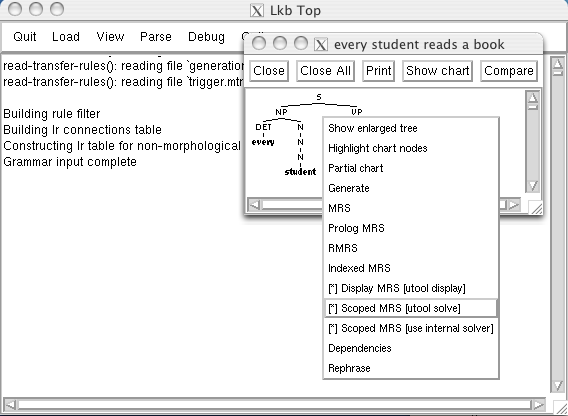
\includegraphics{lkb-integration}
\caption{(caption)}
\label{fig:lkb-integration}
\end{figure}

Utool can be used as a drop in replacement for the MRS constraint
solver built into the LKB system. The distribution contains a Lisp
file \verb|lkb-utool.lisp| that can be simply loaded into a running
LKB session and replaces the internal constraint solver.

Alternatively, the file \verb|lkb-utool-menu.lisp| can be loaded into
a running LKB session, which extends the context menu which shows up
when clicking on a parse tree with two commands:

In both cases, utool has to run in server mode listening in the
standard port 2802.

\subsection{Writing your own client for the Utool Server}

The following perl script illustrates how to implement a utool client.
The script assumes that an utool process runs in server mode on the
local machine listening on the standard port 2802.

\begin{verbatim}
use IO::Socket;

# read a dominance constraint
$message = join('', <>);

# open connection
$socket = IO::Socket::INET->new("localhost:2802") or die $!;

# and send it to the server
print $socket <<EOF;
<utool cmd='solve' output-codec='term-oz'>
  <usr codec='domcon-oz' string='$message'/>
</utool>
EOF

# shutdown connection
$socket->shutdown(1);

# print the answer 
while (<$socket>) { print }
\end{verbatim}

The script reads a dominance constraint from standard input, opens a
connection to the server and sends the dominance constraint to the
server. The answer -- in this case a list of solved forms -- is then
printed to the standard output.

A slightly extended version of the above script can be found
\todo{wo?}.


%%% Local Variables: 
%%% mode: latex
%%% TeX-master: "0"
%%% TeX-command-default: "LaTeX"
%%% End: 


\section{Utool in Practice} \label{sec:practice}

We conclude this documentation with some examples for using Utool in
practice. We will start with some tips on how to use Utool
efficiently. Then we will describe a scenario which we have applied a
lot in our papers \cite{FucKolNieTha04,FliKolTha05,KolTha05b}: running
Utool on all MRS descriptions from a HPSG treebank. This second point
will also contain a runtime comparison between Utool and other
underspecification solvers (including the older C++ version of
Utool). \todo{update this}

\subsection{Some practical tips} \label{sec:practice-some-practical-tips}

\begin{enumerate}
\item \textit{Running Utool in server mode.} \todo{write me}


\item \textit{Running Java in server mode.} The Sun implementation of the
Java VM can run in either ``client'' or ``server'' mode. The client
mode is the default, but if you have a long-running process, the
server mode can be significantly more efficient because it
just-in-time compiles and optimises the Java bytecode more
aggressively.

For optimum performance of Utool, we recommend that you run the JVM in
server mode by calling it as follows:
\begin{verbatim}
$ java -server -jar Utool.jar ...
\end{verbatim}
%$

Because of the increased time for startup and compilation, this works
best if you also run Utool in server mode and send it commands via a
socket, because this gives you the most profit out of the JIT
compilation (Utool needs to solve 3--4 USRs to ``warm up'' until it
achieves optimal performance) and eliminates the startup time.

\begin{figure}
\begin{center}
\todo{runtimes for solving chains using server mode and client mode}
\end{center}
\caption{Runtimes for the command \texttt{solve -n -s -I chain
<length>}, running the Java VM in client and server
mode. \label{fig:chains-server-client}}
\end{figure}


\item \textit{Memory consumption.} The chart that Utool computes for
large USRs can grow to eat up quite a bit of your memory. If it grows
larger than the heap limit of the Java VM, Java will throw an
\verb?OutOfMemoryError? and terminate the process. For most USRs that
you will encounter in practice (including almost all USRs in the HPSG
treebanks), the default limit of 256 MB will be sufficient. However,
for those cases where more memory is needed (e.g.\
\verb?rondane-650.mrs.pl? in the examples directory, which has about
$2 \cdot 10^{12}$ solved forms), you can allow Java to use more heap
space by calling it with the \verb?-Xmx512m? option.

\item \textit{XML character entities.} The Utool Server takes commands
as well-formed XML strings, so it expects you to encode special
characters in the USR as XML character entities. You are probably
familiar with having to replace the \"\ character by \verb?&quot;?
etc., and performing the inverse replacement when decoding the
server's responses.

A lesser known aspect of this, however, is that XML parsers will
ignore whitespace within attribute values according to the XML
specification. In particular, you may use newline characters within a
USR, but these characters will be ignored by the parser. If the
concrete syntax of an input codec requires that there are newlines
(e.g.\ to terminate a comment line in the domcon-oz codec), you must
encode this newline character as the character entity \verb?&#xA;?.
\end{enumerate}




\subsection{Writing your own client for the Utool Server}
\label{sec:practice-client}

It often makes sense to run Utool in server mode. In these cases, you
will probably want to implement a client in your own application that
communicates with the server. This is documented in
Section~\ref{sec:operations-server}, but here we give you the source
code of a minimal client written in Perl. This script assumes that a
Utool Server is running on the local machine on the standard port
2802. It will read a USR in \verb?domcon-oz? format from standard
input or a file and send it to the server as the argument of a
\verb?solve? command. It will then wait for an answer from the server
(i.e., a list of solved forms in \verb?term-oz? format) and print it
to standard out.

\begin{verbatim}
use IO::Socket;

# read a dominance constraint
$message = join('', <>);

# open connection
$socket = IO::Socket::INET->new("localhost:2802") or die $!;

# and send it to the server
print $socket <<EOF;
<utool cmd='solve' output-codec='term-oz'>
  <usr codec='domcon-oz' string='$message'/>
</utool>
EOF

# shutdown output side of the socket
$socket->shutdown(1);

# print the answer 
while (<$socket>) { print }
\end{verbatim}
%$

The key point here is that the client shuts down the side of the
socket that is used to send data from the client to the server. This
tells the server that the input is now complete and it should start
processing it.

An extended version of this script (also in Perl) is part of the
standard Utool distribution and can be found in the directory
\url{projects/Domgraph/tools/client}. 




\subsection{Integration with the LKB Workbench}
\label{sec:integration-lkb}


Utool can be used as a drop-in replacement for the MRS solver built
into the LKB grammar development system \cite{Copestake:LKB-Book},
which is freely available at \todo{URL}. This means that users of the
LKB now have easy access to our solver, which is considerably faster
than the original MRS solver. The integration between LKB and Utool is
achieved via two Lisp source files that we distribute in the directory
\url{projects/Domgraph/tools/lkb}.

If you load the file \verb|lkb-utool.lisp| into the Lisp console
of a running LKB system, the internal MRS solver is replaced by
Utool. Technically, this file defines a function that sends the MRS
(in \verb?mrs-prolog? syntax) to a Utool Server running on the local
machine on port 2802. It will then receive the solved forms from the
server, in \verb?plugging-lkb? syntax, and pass them back to LKB.

 Alternatively, if you load the file \verb|lkb-utool-menu.lisp|
into the Lisp console, two new commands are added to the context menu
for parse trees (see Fig.~\ref{fig:lkb-integration}). The command
``Scoped MRS (utool solve)'' calls Utool to compute all scopings of
the MRS for this parse tree, in the same way as just described. On the
other hand, the ``Display MRS'' command will ask the Utool Server to
perform a \verb?display? command for the given MRS. You can then solve
and further manipulate the USR from the GUI. As before, these commands
also make the assumption that a Utool Server is running on the local
machine, port 2802.


\begin{figure}
\begin{center}
%HEVEA \imgsrc{lkb-integration.png}
%HEVEA \begin{latexonly}
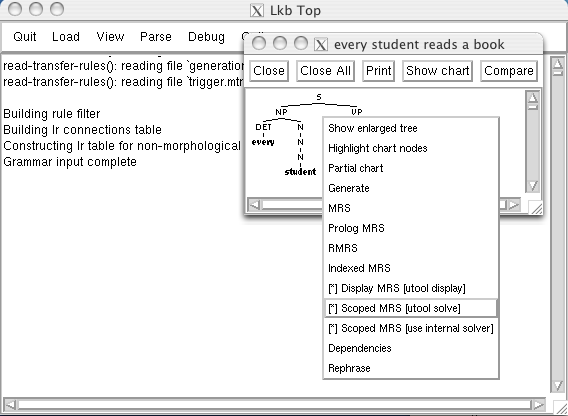
\includegraphics[width=0.8 \textwidth]{lkb-integration}
%HEVEA \end{latexonly}
\end{center}
\caption{Calling Utool from an LKB context menu.
\label{fig:lkb-integration}}
\end{figure}


\subsection{Extracting USRs from a HPSG treebank}
\label{sec:treebank}

The English Resource Grammar (ERG; \citeNP{Copestake&Flickinger:LKB})
is distributed together with a collection of hand-annotated
``Redwoods-style'' corpora that pair for each sentence from the corpus
the preferred syntactic analysis, together with a corresponding
semantic representation based upon MRS. These corpora are extremely
valuable resources because corpora with deep semantic information are
so very rare, and we have occasionally used them in experiments
\cite{FucKolNieTha04,FliKolTha05}.

In order to use the MRSs in these treebanks from within Utool, it is
necessary to extract them from the treebank and save them in
individual files. This can be done by using the script
\verb|extract-gold.lisp|, which can be found in the directory
\url{projects/Domgraph/tools/lkb} in the Utool jar file. Proceed as
follows:

\begin{enumerate}
\item Start the LKB system.
\item Locate the treebank file on your filesystem. Here we will assume
that we are working with the Rondane treebank, which is in
\url{erg/gold/rondane/result} under the main LKB directory. You may
have to unzip the file \verb?result.gz? that comes with the original
ERG distribution first.
\item Run the following commands in the LKB's Lisp console:
\begin{verbatim}
(load "extract-gold")
(utool::extract-prolog "erg/gold/rondane/result" "target-directory")
\end{verbatim}
You need to replace \verb?target-directory? with the name of the
directory in which you want the individual MRSs stored. This will
create a number of files with the extension \verb?.mrs.pl?, one for
each sentence in the treebank. These files are suitable for reading
with the \verb?mrs-prolog? input codec.
\item If you want MRSs in XML format instead, call
\verb?utool::extract-xml? rather than
\verb?utool::extract-prolog?. The arguments of both calls are the
same. 
\item If you pass the additional argument \verb?:solve t? to the
\verb?extract-prolog? call, the MRS constraint solver is applied to
each MRS expression, and the number of fully scoped MRS expressions is
stored in a file \verb|log| in the target directory. This can be
useful to compare the results of the MRS solver and Utool, but can
take quite a while.
\end{enumerate}

The \verb?extract? functions that we distribute will work with the
Rondane treebank \todo{and others}. They will not work directly with
the Redwoods corpus \cite{Oepen&al:Redwoods} because it uses a
slightly different internal format. Use the \texttt{itdsb} (REF)
environment instead.

\todo{This is not very clear yet:
\begin{itemize}
\item What corpora exactly can we convert with the tool in the
distribution?  Only Rondane, or does JH work too? What do I have to do
in order to get these corpora? 
\item What do I have to do to extract the MRSs in the Redwoods corpus?
Where do I get Redwoods? Why are Rondane etc.\ called
``Redwoods-style'' if their internal formats are not compatible?
\end{itemize}
}



\subsection{Benchmarks}

Utool is the fastest solver for underspecified descriptions in the
formalisms of dominance constraints, dominance graphs, Hole Semantics,
and MRS that exists today. This is supported by theoretical complexity
results
\cite{Althaus-J.Algo.,bodirsky-weakly-normal-constraints,KolTha05b},
and we have previously claimed practical efficiency in various
publications.

We will now sketch how such claims of practical efficiency can be
substantiated. In doing so, we will also establish the fact that the
Java implementation of Utool 3.0 is not slower than the earlier C++
implementations of Utool under Linux and Windows, and is in fact a
little faster on Windows. (The same is not currently true on current
Macs, because the PowerPC implementation of Java seems to be very
slow. We hope to obtain comparable runtimes on the new Intel Macs.)

\begin{figure}
%HEVEA \begin{latexonly}
\begin{tabular}{cc}
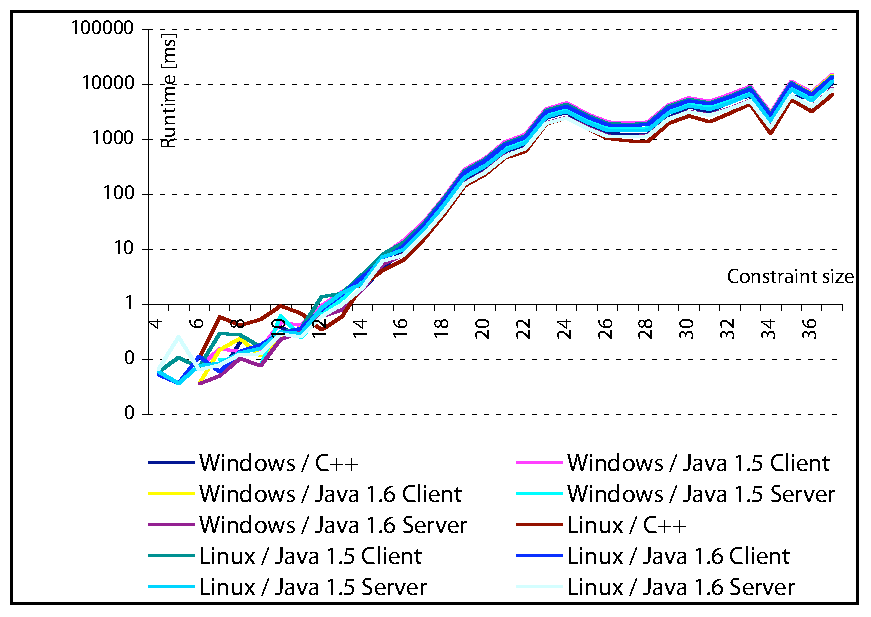
\includegraphics[width=0.4\textwidth]{jh-extraction-mean}
&
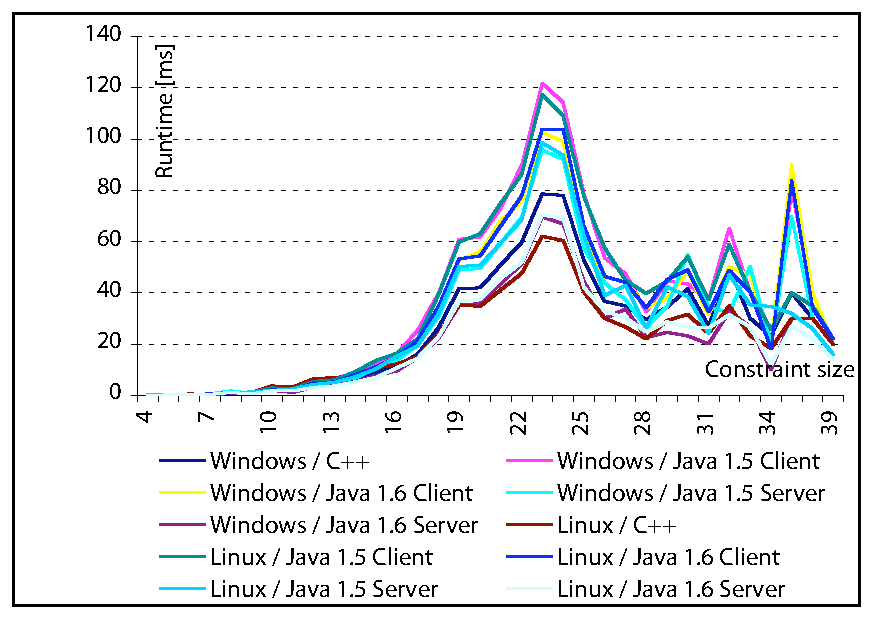
\includegraphics[width=0.4\textwidth]{jh-chart-mean}
\end{tabular}
%HEVEA \end{latexonly}
%HEVEA \imgsrc{jh-extraction-mean.png}
%HEVEA \imgsrc{jh-chart-mean.png}
\caption{Runtimes for the commands \texttt{solvable} and \texttt{solve -n}
of Utool 2.0.1 (C++) and 3.0 (Java) on Windows and Linux. \label{fig:runtimes}}
\end{figure}

As our benchmark example, we chose the Jotenheimen corpus, which is
\todo{what exactly? how many sentences?}. We extracted the MRS
descriptions for each sentence with at most one million solved forms
as described in Section~\ref{sec:treebank}. Then we ran the commands
\verb?utool solvable? (measuring how long it takes to compute the
chart and count all solved forms) and \verb?utool solve -n? (measuring
how long it takes to compute the chart and then extract all solved
forms, without actually encoding or displaying them). We did this
using both Utool 2.0.1 (the last C++ version) and Utool 3.0 (the new
Java version) on all sentences. We ran Utool 3.0 in server mode (using
the \verb?utool server?) to eliminate the overhead for starting up the
JVM.

We performed the benchmarks using a machine with a Pentium M processer
at 1.6 GHz, both on Windows XP Professional and on Linux 2.6.10. Utool
2.0.1 was compiled with Gnu C++ 4.0 under Linux and with the C++
compiler from the Microsoft Visual C++ Toolkit 2003. We ran Utool 3.0
both using Java SE 5.0 and using a beta version of Java SE 6.0; in
both cases, we ran the JVM both in client and in server mode (with the
\verb?-server? JVM flag).

The results of these benchmarks are shown in
Fig.~\ref{fig:runtimes}. Both charts plot the size of the
underspecified description (number of fragments in the dominance
graph) on the X axis and the mean runtime for USRs of this size on the
Y axis. The Y axis is logarithmic in both cases. Looking at the
charts, we can make the following observations:
\begin{itemize}
\item The mean time for computing a chart is dramatically lower than
the time for enumerating all solved forms. This is unsurprising, as
the larger USRs can have hundreds of thousands of solved forms,
whereas the charts remain much smaller.
\item Running Java in server mode is generally much faster than
running it in client mode.
\item Even the beta version of Java 6.0 is noticeably more efficient
than Java 5.0.
\item The difference in performance between Utool 2.0.1 and Utool 3.0
running on Java 6.0 in server mode is negligible under Linux. Under
Windows, the Java version is more efficient (perhaps because we didn't
switch on all the right optimisations in the Visual C++ compiler).
\end{itemize}





\todo{number of sfs vs. chart sizes}





%%% Local Variables: 
%%% mode: latex
%%% TeX-master: "0"
%%% TeX-command-default: "LaTeX"
%%% End: 

%!TEX root = 0.tex

\section{Building Utool} \label{sec:building}

So far, we have focused on how to use the complete Utool system as you
download it, unchanged. This is sufficient in many scenarios -- you
can access Utool from the command line, you can connect to it as a
server, and you can even implement your own Java classes that use our
classes directly, as long as you simply add \verb?Utool.jar? to your
classpath. But there may be a point at which you want to recompile
Utool. For such cases, we will now document how to unpack the Utool
source distribution and recompile it.

The Jar file \verb?Utool-<version>.jar? which you probably downloaded
from the website only contains the compiled class files that are
necessary for running the programme. This is the standard distribution
because it is pretty small, and thus downloads and loads quickly.

If you want to recompile (parts of) Utool, you will need to download
the source distribution. The source distribution has a filename of the
form \verb?Utool-src-<version>.jar?, and is some 4 megabytes in
size. In addition to the Utool classes, it contains the source code of
Utool, all classes of the iText, JGraphT, JGraph, and Getopt libraries
that we use, and the javacc and testng Jars that are used in compiling
Utool. The files in the source distribution Jar are in exactly the
same locations as in the ordinary Jar, so in particular you can use
the command \verb?java -jar Utool-src-<version>.jar? to run Utool. In
addition, you need the Java JDK 5.0 or higher, and you need Apache Ant
1.6 or higher.

Recompilation of Utool from the source distribution proceeds as
follows:

\begin{enumerate}
\item Unpack the Jar file in a new directory:
\begin{verbatim}
$ jar xf Utool-src-<version>.jar
\end{verbatim}
%$

\item Prepare for compiling by moving all files to the directories
where the build script expects them:
\begin{verbatim}
$ ant prepare
\end{verbatim}
%$

\item Change or add classes as you like. The source code of all
classes is under the directory \verb?src?. If you add new classes, you
may have to edit the Ant build script in \url{build.xml}.

\item Recompile as follows:
\begin{verbatim}
$ ant
\end{verbatim}
%$

This will create the file \verb?Utool-<version>.jar? in the directory
\verb?build/lib?, which you can run using \verb?java -jar?  as before.

%\item If you have access to the Jakarta BCEL library (we use
%version 5.1), you can add this library to your classpath and run

%\begin{verbatim}
%$ ant utool-compact
%\end{verbatim}
%$

%to build the (smaller) file \verb?build/lib/Utool-<version>.jar?
%which constitutes the main Utool distribution.
\end{enumerate}






%%% Local Variables: 
%%% mode: latex
%%% TeX-master: "0"
%%% TeX-command-default: "LaTeX"
%%% End: 

%
\section{Further Reading}  \label{sec:further}




%%% Local Variables: 
%%% mode: latex
%%% TeX-master: "0"
%%% TeX-command-default: "LaTeX"
%%% End: 

%!TEX root = 0.tex

\section{Conclusion}  \label{sec:conclusion}

In this document, we have described Utool, the Swiss Army Knife of
Underspecification. In particular, we have explained how to use Utool
and how to extend Utool, and listed some tips and experiences on using
Utool in practice.

As this is the first version of this manual, we are sure that there
are many things that we can improve. We would therefore greatly
appreciate any comments or suggestions that you might have. Please
send them to \url{koller@coli.uni-sb.de}, and we will try to take them
into account for the next version. 

We believe that Utool 3.0 will do a good job at supporting researchers
who work on underspecification. Nevertheless, we will continue to
improve it, and have already started working on version 3.1. This new
version will mostly focus on improvements to the Utool architecture
that won't be immediately visible to the end user. However, we are
also planning to improve the functionality of the Ubench GUI and
implement new codecs. In addition, we would be thrilled to hear your
ideas for things that could be improved, as well as bug
reports. Please send these to \url{koller@coli.uni-sb.de} as well.

We hope you will enjoy using Utool!





%%% Local Variables: 
%%% mode: latex
%%% TeX-master: "0"
%%% TeX-command-default: "LaTeX"
%%% End: 



\bibliographystyle{chicago}
\bibliography{chorus}

\end{document}

